\documentclass[10pt,a4paper]{report}
\usepackage[utf8]{inputenc}
\usepackage[french]{babel}
\usepackage{graphicx}
\usepackage{float}
\usepackage{geometry}
\usepackage{hyperref}
\usepackage{tikz}

\geometry{margin=2cm}

\begin{document}
\begin{center}
\begin{tabular*}{\textwidth}{l @{\extracolsep{\fill}} r}

  
\includegraphics [width=40mm]{../images/ENSEIRB-MATMECA.ps} &
  \raisebox{0.75\height}
           {
\includegraphics [width=40mm]{../images/logo-LaBRI-couleur.ps}}

\end{tabular*}

\vspace{\stretch{1}}


\textsc{\Huge Manuel d'utilisation de PFA-NetHack}\\[0.5cm]

\rule{0.4\textwidth}{1pt}

\vspace{\stretch{1}}

\begin{center}
  
  \begin{flushleft}
    \large
    \emph{Auteurs :}\\
    \begin{itemize}
    \item Benoît Ruelle
    \item David Bitonneau
    \item Ludovic Hofer
    \end{itemize}
  \end{flushleft}
  
  
  \begin{flushright}
    \large
    \emph{Responsables :}\\
    Pédagogique - M.~Renault\\
    Client - M.~Le Borgne\\
  \end{flushright}
\end{center}

\vspace{\stretch{1}}
                  
{\large Deuxième année, filière informatique}

~

{\large 16 octobre 2012 - 29 mars 2013}\\
                  
\end{center}
\thispagestyle{empty}
\pagebreak

\tableofcontents

\chapter{Utilisation du code fourni}
\section{Génération des exécutables}

Un script \verb!nh-setup.sh! permet de télécharger, patcher et compiler le jeu
pour linux avec les modifications apportées dans le cadre du projet.
Avant la compilation, l'utilisateur doit répondre à quelques questions rapides
pour renseigner les patchs qu'il souhaite appliquer. À l'issue de la
compulation, le jeu sera installé dans le répertoire courrant.

\textbf{TODO: David} configuration des patchs appliqués par défaut?

Certains des bots fournis nécessitent d'être compilés avant de pouvoir être
utilisés. C'est le cas des bots écrits en Java.



\section{Paramétrer l'exécution de NetHack}

Des variables d'environnement peuvent être utilisées pour modifier le
comportement du jeu :

\begin{itemize}
\item \verb!NH_MM_SOCKPATH! : spécifier un chemin pour la socket unix (permettant la communication entre NetHack et les bots) à créer. Par défaut, le middleman créé \emph{/tmp/mmsock}.
\item \verb!NH_MM_DUPMSGS! : si mise à une valeur différente de 0, cette
	variable active la duplication des messages envoyées au bot sur la sortie
	standard (peut être utilisé pour rediriger vers \verb!bots/dummy-client.pl!).
	Désactivée par défaut.
\item \verb!NH_MM_LOGGING! : si mise à une valeur différente de 0, cette variable active l'enregistrement de logs du middleman dans le fichier \emph{nethackdir/mm.log}. Désactivée par défaut.
\item \verb!NH_MM_TIMEOUT! : spécifie le timeout en secondes pour les communications avec le bot. Si le bot met un temps en secondes supérieur à cette valeur, le middleman quitte la partie. Par défaut, cette variables est mise à 2 secondes.
\item \verb!NH_MAX_MOVES! :
  Ce paramètre spécifie le nombre de mouvement maximal autorisé au bot, sachant
  que le bot n'est pas sensé mourir, c'est la définition de ce paramètre qui
  spécifiera la durée de la partie. Par défaut, cette variable vaut 20000.
\item \verb!NH_DATABASE_PATH! :
  Spécifie le chemin d'accès pour la base de données à laquelle les résultats
  seront ajoutés. Par défaut, ce chemin vaut \emph{/tmp/test.db}.
\item \verb!NH_BOT_NAME! :
  Permet d'indiquer le nom du bot afin d'ajouter une entrée complète à la base
  de données. Par défaut : la valeur est \emph{unknown}.
\item \verb!NH_MODE_NAME! :
  Permet d'indiquer le nom du mode utilisé afin de l'ajouter correctement à la
  base de données. Par défaut : la valeur est \emph{seek\_secret}.
\item \verb!NH_SEED! :
  Permet de donner la valeur de la graine à utiliser pour l'initialisation du
  générateur de nombres aléatoires de NetHack. Par défaut, si cette
  valeur n'est pas spécifiée, la graine utilisée est une combinaison du nombre
  de secondes et de millisecondes écoulées depuis l'epoch.
\end{itemize}

\section{Lancer une partie}

\subsection{Lancement manuel}

Tout d'abord, le jeu doit être lancé (avec les paramètres nécessaires) avant le bot. NetHack attendra alors qu'un bot se connecte. Le bot choisi ou le dummy-client peuvent alors être lancés manuellement.

\subsection{Lancer plusieurs parties grâce à un script}
Le script \emph{game\_runner.sh} permet à l'utilisateur de lancer facilement
un grand nombre de parties qui ne diffèrent que par la graine aléatoire
utilisée.
\\
Il est possible de lancer plusieurs instances de ce script en simultané, et ce
même si elles enregistrent leurs résultats dans la même base de donnée. Chaque
script créé un dossier dans \emph{/tmp/} avant d'y copier le code de NetHack ainsi que
le bot, ceci permet de continuer à travailler sur les bots ou sur le code de
NetHack sans risquer d'interférer avec les parties déjà lancées. Si ce
comportement n'est pas souhaité, il est relativement simple de commenter la
partie du code qui y est associé.
\\
Plusieurs options peuvent être utilisées pour ce script, il est possible
d'obtenir plus de détails facilement en utilisant la commande suivante :
\emph{game\_runner.sh -h}.

\section{Remplir une base de donnée}
Le script \emph{data\_builder.sh} permet de générer facilement une base de
données contenant les résultats d'un grand nombre de parties. Ce script n'est
pas paramétré, mais il est aisément modifiable à la main, son but est
principalement de fournir une base pour permettre à un utilisateur novice
d'ajouter ou de supprimer des bots où des nombres de mouvements autorisés à
l'ensemble des parties à lancer.
\\
Bien que lui même ne lance pas plusieurs processus, ce script peut
parfaitement être exécuté $N$ fois, $N$ étant le nombre de processeur
disponible. Cependant l'affichage n'a pas été prévu pour gérer plusieurs
processus à l'aide d'un seul terminal, ainsi, si l'on souhaite observer
l'évolution des exécutions, il est conseillé des les exécuter dans $N$
terminaux différents.


\section{Voir ou revoir une partie}

En mettant la variable d'environnement \verb!NH_MM_DUPMSGS! à une valeur
différente de 0 lors du lancement du jeu, le middleman dupliquera tous les
messages envoyés au bot vers la sortie standard. Cette sortie peut être
redirigée vers le programme \verb!bots/dummy-client.pl! qui s'exécutera alors en
'lecture seule' \footnote{\verb!bots/dummy-client.pl! a plusieurs modes
d'exécution} et interprétera le flux pour afficher la carte correspondante à
la partie en cours. Exemple d'exécution :

\begin{verbatim}
# Dans un premier terminal :
$ NH_MM_DUPMSGS=1 ./nethack-3.4.3/nethack 2> /dev/null 1| perl bots/dummy-client.pl

# Dans un second (utiliser le bot au choix) :
$ java -jar bots/diffusion/Bot.jar
# Ou même (dummy-client utilisé dans un second mode) :
$ perl bots/dummy-client.pl
\end{verbatim}


En redirigeant cette sortie vers un fichier (ou en lançant le script
\verb!game_runner.sh! avec l'option \verb!-r!), le déroulement de la partie peut
être sauvegardée.  Le programme \verb!viewer/viewer.pl! permet d'exploiter
cette sauvegarde afin de visualiser la partie a posteriori. Voir le README
correspondant. Exemple :

\begin{verbatim}
$ NH_MM_DUPMSGS=1 ./nethack-3.4.3/nethack > replay
# Puis, une fois la partie terminée
$ perl viewer/viewer.pl replay
\end{verbatim}


\section{Aperçu du comportement d'un bot}

\paragraph{}
Une sauvegarde peut également être interprété par le
programme \verb!viewer/toTikZ.pl! qui génère une carte donnant un apperçu du
nombre de tours passés sur chaque case des niveaux visités. Utilisé sans
option, ce programme ne génèrera que la portion de code TikZ correspondant à
la carte. Utilisé avec l'option \verb!-f!, un document latex complet qui peut
alors être passé à \verb!pdflatex! sera généré.
L'option \verb!-e! de ce programme génère un autre type de carte
qui permet de visualiser l'ordre dans lequel s'est faite l'exploration.

\begin{figure}[h]
	\caption{Nombre de visites sur chaque case sur deux niveaux du starter package java. En blanc les cases non visitées, en jaune clair les cases visitées peu de fois, en rouge les cases visitées un grand nombre de fois.}
	\resizebox{\columnwidth}{!}{\begin{tikzpicture}[scale=0.3]
\node at (2, -27) {\verb!-!};
\node at (3, -27) {\verb!-!};
\node at (4, -27) {\verb!-!};
\node at (5, -27) {\verb!-!};
\node at (6, -27) {\verb!-!};
\node at (7, -27) {\verb!-!};
\node at (8, -27) {\verb!-!};
\node at (9, -27) {\verb!-!};
\node at (10, -27) {\verb!-!};
\node at (11, -27) {\verb!-!};
\node at (21, -27) {\verb!-!};
\node at (22, -27) {\verb!-!};
\node at (23, -27) {\verb!-!};
\node at (24, -27) {\verb!-!};
\node at (25, -27) {\verb!-!};
\node at (26, -27) {\verb!-!};
\node at (27, -27) {\verb!-!};
\node at (28, -27) {\verb!-!};
\node at (29, -27) {\verb!-!};
\node at (30, -27) {\verb!-!};
\node at (31, -27) {\verb!-!};
\node at (32, -27) {\verb!-!};
\node at (33, -27) {\verb!-!};
\node at (34, -27) {\verb!-!};
\node at (35, -27) {\verb!-!};
\node at (2, -28) {\verb!|!};
\node [fill=red!44!yellow] at (3, -28) {\verb!.!};
\node [fill=red!57!yellow] at (4, -28) {\verb!.!};
\node [fill=red!51!yellow] at (5, -28) {\verb!.!};
\node [fill=red!53!yellow] at (6, -28) {\verb!.!};
\node [fill=red!56!yellow] at (7, -28) {\verb!.!};
\node [fill=red!57!yellow] at (8, -28) {\verb!.!};
\node [fill=red!49!yellow] at (9, -28) {\verb!.!};
\node [fill=red!33!yellow] at (10, -28) {\verb!.!};
\node at (11, -28) {\verb!|!};
\node at (21, -28) {\verb!|!};
\node [fill=red!11!yellow] at (22, -28) {\verb!.!};
\node [fill=red!11!yellow] at (23, -28) {\verb!.!};
\node [fill=red!13!yellow] at (24, -28) {\verb!.!};
\node [fill=red!7!yellow] at (25, -28) {\verb!.!};
\node [fill=red!6!yellow] at (26, -28) {\verb!.!};
\node [fill=red!6!yellow] at (27, -28) {\verb!.!};
\node [fill=red!6!yellow] at (28, -28) {\verb!.!};
\node [fill=red!4!yellow] at (29, -28) {\verb!.!};
\node [fill=red!3!yellow] at (30, -28) {\verb!.!};
\node [fill=red!9!yellow] at (31, -28) {\verb!.!};
\node [fill=red!6!yellow] at (32, -28) {\verb!.!};
\node [fill=red!4!yellow] at (33, -28) {\verb!.!};
\node [fill=red!3!yellow] at (34, -28) {\verb!.!};
\node at (35, -28) {\verb!|!};
\node at (2, -29) {\verb!|!};
\node [fill=red!68!yellow] at (3, -29) {\verb!.!};
\node [fill=red!79!yellow] at (4, -29) {\verb!.!};
\node [fill=red!95!yellow] at (5, -29) {\verb!.!};
\node [fill=red!97!yellow] at (6, -29) {\verb!.!};
\node [fill=red!83!yellow] at (7, -29) {\verb!.!};
\node [fill=red!100!yellow] at (8, -29) {\verb!.!};
\node [fill=red!69!yellow] at (9, -29) {\verb!.!};
\node [fill=red!59!yellow] at (10, -29) {\verb!.!};
\node [fill=red!36!yellow] at (11, -29) {\verb!.!};
\node [fill=red!16!yellow] at (12, -29) {\verb!#!};
\node [fill=red!15!yellow] at (13, -29) {\verb!#!};
\node [fill=red!13!yellow] at (14, -29) {\verb!#!};
\node at (21, -29) {\verb!|!};
\node [fill=red!16!yellow] at (22, -29) {\verb!.!};
\node [fill=red!20!yellow] at (23, -29) {\verb!.!};
\node [fill=red!14!yellow] at (24, -29) {\verb!.!};
\node [fill=red!16!yellow] at (25, -29) {\verb!.!};
\node [fill=red!12!yellow] at (26, -29) {\verb!.!};
\node [fill=red!10!yellow] at (27, -29) {\verb!.!};
\node [fill=red!6!yellow] at (28, -29) {\verb!.!};
\node [fill=red!6!yellow] at (29, -29) {\verb!.!};
\node [fill=red!8!yellow] at (30, -29) {\verb!.!};
\node [fill=red!8!yellow] at (31, -29) {\verb!.!};
\node [fill=red!10!yellow] at (32, -29) {\verb!.!};
\node [fill=red!8!yellow] at (33, -29) {\verb!.!};
\node [fill=red!6!yellow] at (34, -29) {\verb!.!};
\node at (35, -29) {\verb!|!};
\node at (2, -30) {\verb!|!};
\node [fill=red!60!yellow] at (3, -30) {\verb!.!};
\node [fill=red!94!yellow] at (4, -30) {\verb!.!};
\node [fill=red!75!yellow] at (5, -30) {\verb!.!};
\node [fill=red!86!yellow] at (6, -30) {\verb!.!};
\node [fill=red!89!yellow] at (7, -30) {\verb!.!};
\node [fill=red!92!yellow] at (8, -30) {\verb!.!};
\node [fill=red!89!yellow] at (9, -30) {\verb!.!};
\node [fill=red!58!yellow] at (10, -30) {\verb!.!};
\node at (11, -30) {\verb!|!};
\node [fill=red!25!yellow] at (14, -30) {\verb!#!};
\node [fill=red!16!yellow] at (20, -30) {\verb!#!};
\node [fill=red!22!yellow] at (21, -30) {\verb!.!};
\node [fill=red!19!yellow] at (22, -30) {\verb!.!};
\node [fill=red!16!yellow] at (23, -30) {\verb!.!};
\node [fill=red!20!yellow] at (24, -30) {\verb!.!};
\node [fill=red!13!yellow] at (25, -30) {\verb!.!};
\node [fill=red!10!yellow] at (26, -30) {\verb!.!};
\node [fill=red!10!yellow] at (27, -30) {\verb!.!};
\node [fill=red!8!yellow] at (28, -30) {\verb!.!};
\node [fill=red!8!yellow] at (29, -30) {\verb!.!};
\node [fill=red!5!yellow] at (30, -30) {\verb!.!};
\node [fill=red!8!yellow] at (31, -30) {\verb!.!};
\node [fill=red!6!yellow] at (32, -30) {\verb!.!};
\node [fill=red!13!yellow] at (33, -30) {\verb!.!};
\node [fill=red!7!yellow] at (34, -30) {\verb!.!};
\node at (35, -30) {\verb!|!};
\node at (41, -30) {\verb!-!};
\node at (42, -30) {\verb!-!};
\node at (43, -30) {\verb!-!};
\node at (44, -30) {\verb!-!};
\node at (45, -30) {\verb!-!};
\node at (2, -31) {\verb!|!};
\node [fill=red!43!yellow] at (3, -31) {\verb!.!};
\node [fill=red!63!yellow] at (4, -31) {\verb!.!};
\node [fill=red!63!yellow] at (5, -31) {\verb!.!};
\node [fill=red!54!yellow] at (6, -31) {\verb!.!};
\node [fill=red!58!yellow] at (7, -31) {\verb!.!};
\node [fill=red!62!yellow] at (8, -31) {\verb!.!};
\node [fill=red!51!yellow] at (9, -31) {\verb!.!};
\node [fill=red!29!yellow] at (10, -31) {\verb!.!};
\node at (11, -31) {\verb!|!};
\node [fill=red!18!yellow] at (14, -31) {\verb!#!};
\node [fill=red!29!yellow] at (15, -31) {\verb!#!};
\node [fill=red!18!yellow] at (16, -31) {\verb!#!};
\node [fill=red!13!yellow] at (18, -31) {\verb!#!};
\node [fill=red!27!yellow] at (19, -31) {\verb!#!};
\node [fill=red!20!yellow] at (20, -31) {\verb!#!};
\node at (21, -31) {\verb!|!};
\node [fill=red!18!yellow] at (22, -31) {\verb!.!};
\node [fill=red!20!yellow] at (23, -31) {\verb!.!};
\node [fill=red!18!yellow] at (24, -31) {\verb!.!};
\node [fill=red!9!yellow] at (25, -31) {\verb!.!};
\node [fill=red!4!yellow] at (26, -31) {\verb!.!};
\node [fill=red!4!yellow] at (27, -31) {\verb!.!};
\node [fill=red!6!yellow] at (28, -31) {\verb!.!};
\node [fill=red!4!yellow] at (29, -31) {\verb!.!};
\node [fill=red!3!yellow] at (30, -31) {\verb!.!};
\node [fill=red!2!yellow] at (31, -31) {\verb!.!};
\node [fill=red!9!yellow] at (32, -31) {\verb!.!};
\node [fill=red!6!yellow] at (33, -31) {\verb!.!};
\node [fill=red!4!yellow] at (34, -31) {\verb!.!};
\node at (35, -31) {\verb!|!};
\node at (41, -31) {\verb!|!};
\node [fill=red!7!yellow] at (42, -31) {\verb!.!};
\node [fill=red!12!yellow] at (43, -31) {\verb!.!};
\node [fill=red!10!yellow] at (44, -31) {\verb!.!};
\node at (45, -31) {\verb!|!};
\node at (2, -32) {\verb!-!};
\node at (3, -32) {\verb!-!};
\node [fill=red!41!yellow] at (4, -32) {\verb!.!};
\node at (5, -32) {\verb!-!};
\node at (6, -32) {\verb!-!};
\node at (7, -32) {\verb!-!};
\node at (8, -32) {\verb!-!};
\node at (9, -32) {\verb!-!};
\node at (10, -32) {\verb!-!};
\node at (11, -32) {\verb!-!};
\node [fill=red!31!yellow] at (16, -32) {\verb!#!};
\node [fill=red!31!yellow] at (18, -32) {\verb!#!};
\node at (21, -32) {\verb!-!};
\node at (22, -32) {\verb!-!};
\node [fill=red!12!yellow] at (23, -32) {\verb!.!};
\node at (24, -32) {\verb!-!};
\node at (25, -32) {\verb!-!};
\node at (26, -32) {\verb!-!};
\node at (27, -32) {\verb!-!};
\node at (28, -32) {\verb!-!};
\node at (29, -32) {\verb!-!};
\node at (30, -32) {\verb!-!};
\node at (31, -32) {\verb!-!};
\node at (32, -32) {\verb!-!};
\node at (33, -32) {\verb!-!};
\node at (34, -32) {\verb!-!};
\node at (35, -32) {\verb!-!};
\node at (41, -32) {\verb!|!};
\node [fill=red!10!yellow] at (42, -32) {\verb!.!};
\node [fill=red!24!yellow] at (43, -32) {\verb!.!};
\node [fill=red!17!yellow] at (44, -32) {\verb!.!};
\node at (45, -32) {\verb!|!};
\node at (72, -32) {\verb!|!};
\node [fill=red!16!yellow] at (4, -33) {\verb!#!};
\node [fill=red!24!yellow] at (5, -33) {\verb!#!};
\node [fill=red!11!yellow] at (6, -33) {\verb!#!};
\node [fill=red!9!yellow] at (7, -33) {\verb!#!};
\node [fill=red!12!yellow] at (8, -33) {\verb!#!};
\node [fill=red!6!yellow] at (9, -33) {\verb!#!};
\node [fill=red!15!yellow] at (16, -33) {\verb!#!};
\node [fill=red!40!yellow] at (17, -33) {\verb!#!};
\node [fill=red!21!yellow] at (18, -33) {\verb!#!};
\node [fill=red!3!yellow] at (23, -33) {\verb!#!};
\node [fill=red!4!yellow] at (24, -33) {\verb!#!};
\node [fill=red!4!yellow] at (25, -33) {\verb!#!};
\node [fill=red!2!yellow] at (26, -33) {\verb!#!};
\node at (39, -33) {\verb!#!};
\node at (40, -33) {\verb!#!};
\node at (41, -33) {\verb!+!};
\node [fill=red!14!yellow] at (42, -33) {\verb!.!};
\node [fill=red!21!yellow] at (43, -33) {\verb!.!};
\node [fill=red!21!yellow] at (44, -33) {\verb!.!};
\node at (45, -33) {\verb!|!};
\node [fill=red!6!yellow] at (46, -33) {\verb!#!};
\node [fill=red!8!yellow] at (47, -33) {\verb!#!};
\node [fill=red!6!yellow] at (48, -33) {\verb!#!};
\node [fill=red!1!yellow] at (49, -33) {\verb!#!};
\node [fill=red!0!yellow] at (50, -33) {\verb!#!};
\node at (51, -33) {\verb!#!};
\node at (68, -33) {\verb!.!};
\node at (69, -33) {\verb!.!};
\node at (70, -33) {\verb!.!};
\node at (71, -33) {\verb!.!};
\node at (72, -33) {\verb!|!};
\node [fill=red!17!yellow] at (9, -34) {\verb!#!};
\node [fill=red!12!yellow] at (16, -34) {\verb!#!};
\node [fill=red!30!yellow] at (18, -34) {\verb!#!};
\node [fill=red!6!yellow] at (26, -34) {\verb!#!};
\node [fill=red!0!yellow] at (39, -34) {\verb!#!};
\node at (41, -34) {\verb!|!};
\node [fill=red!8!yellow] at (42, -34) {\verb!.!};
\node [fill=red!15!yellow] at (43, -34) {\verb!.!};
\node [fill=red!12!yellow] at (44, -34) {\verb!.!};
\node [fill=red!15!yellow] at (45, -34) {\verb!.!};
\node [fill=red!16!yellow] at (46, -34) {\verb!#!};
\node [fill=red!12!yellow] at (47, -34) {\verb!#!};
\node [fill=red!6!yellow] at (48, -34) {\verb!#!};
\node [fill=red!5!yellow] at (49, -34) {\verb!#!};
\node at (72, -34) {\verb!|!};
\node [fill=red!10!yellow] at (9, -35) {\verb!#!};
\node [fill=red!24!yellow] at (10, -35) {\verb!#!};
\node [fill=red!18!yellow] at (11, -35) {\verb!#!};
\node [fill=red!6!yellow] at (16, -35) {\verb!#!};
\node [fill=red!13!yellow] at (18, -35) {\verb!#!};
\node [fill=red!25!yellow] at (19, -35) {\verb!#!};
\node [fill=red!9!yellow] at (20, -35) {\verb!#!};
\node [fill=red!6!yellow] at (26, -35) {\verb!#!};
\node [fill=red!6!yellow] at (27, -35) {\verb!#!};
\node [fill=red!1!yellow] at (28, -35) {\verb!#!};
\node [fill=red!1!yellow] at (37, -35) {\verb!#!};
\node [fill=red!5!yellow] at (38, -35) {\verb!#!};
\node [fill=red!5!yellow] at (39, -35) {\verb!#!};
\node at (41, -35) {\verb!-!};
\node at (42, -35) {\verb!-!};
\node at (43, -35) {\verb!-!};
\node at (44, -35) {\verb!-!};
\node at (45, -35) {\verb!-!};
\node [fill=red!17!yellow] at (46, -35) {\verb!#!};
\node [fill=red!7!yellow] at (49, -35) {\verb!#!};
\node [fill=red!4!yellow] at (51, -35) {\verb!#!};
\node at (58, -35) {\verb!#!};
\node [fill=red!33!yellow] at (11, -36) {\verb!#!};
\node [fill=red!4!yellow] at (16, -36) {\verb!#!};
\node [fill=red!16!yellow] at (20, -36) {\verb!#!};
\node [fill=red!8!yellow] at (23, -36) {\verb!#!};
\node [fill=red!5!yellow] at (24, -36) {\verb!#!};
\node [fill=red!4!yellow] at (25, -36) {\verb!#!};
\node [fill=red!6!yellow] at (26, -36) {\verb!#!};
\node [fill=red!10!yellow] at (27, -36) {\verb!#!};
\node [fill=red!4!yellow] at (28, -36) {\verb!#!};
\node [fill=red!2!yellow] at (29, -36) {\verb!#!};
\node [fill=red!2!yellow] at (30, -36) {\verb!#!};
\node [fill=red!1!yellow] at (31, -36) {\verb!#!};
\node [fill=red!0!yellow] at (32, -36) {\verb!#!};
\node [fill=red!0!yellow] at (33, -36) {\verb!#!};
\node [fill=red!2!yellow] at (34, -36) {\verb!#!};
\node [fill=red!2!yellow] at (35, -36) {\verb!#!};
\node [fill=red!2!yellow] at (36, -36) {\verb!#!};
\node [fill=red!5!yellow] at (37, -36) {\verb!#!};
\node [fill=red!4!yellow] at (38, -36) {\verb!#!};
\node [fill=red!3!yellow] at (39, -36) {\verb!#!};
\node [fill=red!4!yellow] at (40, -36) {\verb!#!};
\node [fill=red!4!yellow] at (41, -36) {\verb!#!};
\node [fill=red!3!yellow] at (42, -36) {\verb!#!};
\node [fill=red!3!yellow] at (43, -36) {\verb!#!};
\node [fill=red!2!yellow] at (44, -36) {\verb!#!};
\node [fill=red!4!yellow] at (45, -36) {\verb!#!};
\node [fill=red!9!yellow] at (46, -36) {\verb!#!};
\node [fill=red!5!yellow] at (47, -36) {\verb!#!};
\node [fill=red!2!yellow] at (48, -36) {\verb!#!};
\node [fill=red!3!yellow] at (49, -36) {\verb!#!};
\node [fill=red!8!yellow] at (50, -36) {\verb!#!};
\node [fill=red!4!yellow] at (51, -36) {\verb!#!};
\node [fill=red!0!yellow] at (58, -36) {\verb!#!};
\node [fill=red!14!yellow] at (11, -37) {\verb!#!};
\node [fill=red!28!yellow] at (12, -37) {\verb!#!};
\node [fill=red!13!yellow] at (13, -37) {\verb!#!};
\node [fill=red!2!yellow] at (16, -37) {\verb!#!};
\node [fill=red!9!yellow] at (20, -37) {\verb!#!};
\node [fill=red!16!yellow] at (21, -37) {\verb!#!};
\node [fill=red!13!yellow] at (22, -37) {\verb!#!};
\node [fill=red!6!yellow] at (23, -37) {\verb!#!};
\node at (24, -37) {\verb!-!};
\node at (25, -37) {\verb!-!};
\node at (26, -37) {\verb!-!};
\node at (27, -37) {\verb!-!};
\node [fill=red!8!yellow] at (28, -37) {\verb!.!};
\node at (29, -37) {\verb!-!};
\node [fill=red!3!yellow] at (35, -37) {\verb!#!};
\node [fill=red!2!yellow] at (36, -37) {\verb!#!};
\node [fill=red!0!yellow] at (37, -37) {\verb!#!};
\node [fill=red!3!yellow] at (51, -37) {\verb!#!};
\node at (53, -37) {\verb!-!};
\node at (54, -37) {\verb!-!};
\node at (55, -37) {\verb!-!};
\node at (56, -37) {\verb!-!};
\node at (57, -37) {\verb!-!};
\node [fill=red!2!yellow] at (58, -37) {\verb!#!};
\node [fill=red!1!yellow] at (9, -38) {\verb!#!};
\node [fill=red!19!yellow] at (13, -38) {\verb!#!};
\node [fill=red!4!yellow] at (16, -38) {\verb!#!};
\node [fill=red!14!yellow] at (22, -38) {\verb!#!};
\node [fill=red!10!yellow] at (23, -38) {\verb!#!};
\node at (24, -38) {\verb!|!};
\node [fill=red!1!yellow] at (25, -38) {\verb!.!};
\node [fill=red!8!yellow] at (26, -38) {\verb!.!};
\node [fill=red!8!yellow] at (27, -38) {\verb!.!};
\node [fill=red!6!yellow] at (28, -38) {\verb!.!};
\node at (29, -38) {\verb!|!};
\node at (35, -38) {\verb!#!};
\node [fill=red!0!yellow] at (51, -38) {\verb!#!};
\node [fill=red!2!yellow] at (52, -38) {\verb!#!};
\node [fill=red!4!yellow] at (53, -38) {\verb!.!};
\node [fill=red!4!yellow] at (54, -38) {\verb!.!};
\node [fill=red!2!yellow] at (55, -38) {\verb!.!};
\node at (56, -38) {\verb!.!};
\node at (57, -38) {\verb!|!};
\node [fill=red!2!yellow] at (58, -38) {\verb!#!};
\node at (6, -39) {\verb!-!};
\node at (7, -39) {\verb!-!};
\node at (8, -39) {\verb!-!};
\node [fill=red!8!yellow] at (9, -39) {\verb!.!};
\node at (10, -39) {\verb!-!};
\node at (11, -39) {\verb!-!};
\node at (12, -39) {\verb!-!};
\node [fill=red!21!yellow] at (13, -39) {\verb!.!};
\node at (14, -39) {\verb!-!};
\node at (15, -39) {\verb!-!};
\node [fill=red!18!yellow] at (16, -39) {\verb!#!};
\node [fill=red!8!yellow] at (22, -39) {\verb!#!};
\node [fill=red!10!yellow] at (23, -39) {\verb!#!};
\node [fill=red!10!yellow] at (24, -39) {\verb!.!};
\node [fill=red!6!yellow] at (25, -39) {\verb!.!};
\node [fill=red!12!yellow] at (26, -39) {\verb!.!};
\node [fill=red!18!yellow] at (27, -39) {\verb!.!};
\node [fill=red!10!yellow] at (28, -39) {\verb!.!};
\node [fill=red!3!yellow] at (29, -39) {\verb!.!};
\node [fill=red!0!yellow] at (30, -39) {\verb!#!};
\node at (31, -39) {\verb!#!};
\node at (53, -39) {\verb!|!};
\node [fill=red!2!yellow] at (54, -39) {\verb!.!};
\node [fill=red!1!yellow] at (55, -39) {\verb!.!};
\node [fill=red!1!yellow] at (56, -39) {\verb!.!};
\node at (57, -39) {\verb!|!};
\node [fill=red!2!yellow] at (58, -39) {\verb!#!};
\node at (6, -40) {\verb!|!};
\node [fill=red!8!yellow] at (7, -40) {\verb!.!};
\node [fill=red!23!yellow] at (8, -40) {\verb!.!};
\node [fill=red!22!yellow] at (9, -40) {\verb!.!};
\node [fill=red!25!yellow] at (10, -40) {\verb!.!};
\node [fill=red!22!yellow] at (11, -40) {\verb!.!};
\node [fill=red!24!yellow] at (12, -40) {\verb!.!};
\node [fill=red!28!yellow] at (13, -40) {\verb!.!};
\node [fill=red!28!yellow] at (14, -40) {\verb!.!};
\node [fill=red!26!yellow] at (15, -40) {\verb!.!};
\node [fill=red!16!yellow] at (16, -40) {\verb!#!};
\node [fill=red!6!yellow] at (23, -40) {\verb!#!};
\node at (24, -40) {\verb!|!};
\node [fill=red!12!yellow] at (25, -40) {\verb!.!};
\node [fill=red!16!yellow] at (26, -40) {\verb!.!};
\node [fill=red!14!yellow] at (27, -40) {\verb!.!};
\node [fill=red!12!yellow] at (28, -40) {\verb!.!};
\node at (29, -40) {\verb!|!};
\node at (53, -40) {\verb!|!};
\node [fill=red!1!yellow] at (54, -40) {\verb!.!};
\node [fill=red!1!yellow] at (55, -40) {\verb!.!};
\node [fill=red!0!yellow] at (56, -40) {\verb!.!};
\node at (57, -40) {\verb!|!};
\node [fill=red!4!yellow] at (58, -40) {\verb!#!};
\node at (6, -41) {\verb!|!};
\node [fill=red!16!yellow] at (7, -41) {\verb!.!};
\node [fill=red!31!yellow] at (8, -41) {\verb!.!};
\node [fill=red!33!yellow] at (9, -41) {\verb!.!};
\node [fill=red!33!yellow] at (10, -41) {\verb!.!};
\node [fill=red!39!yellow] at (11, -41) {\verb!.!};
\node [fill=red!37!yellow] at (12, -41) {\verb!<!};
\node [fill=red!39!yellow] at (13, -41) {\verb!.!};
\node [fill=red!41!yellow] at (14, -41) {\verb!.!};
\node at (15, -41) {\verb!|!};
\node [fill=red!2!yellow] at (23, -41) {\verb!#!};
\node at (24, -41) {\verb!|!};
\node [fill=red!5!yellow] at (25, -41) {\verb!.!};
\node [fill=red!9!yellow] at (26, -41) {\verb!.!};
\node [fill=red!14!yellow] at (27, -41) {\verb!.!};
\node [fill=red!8!yellow] at (28, -41) {\verb!.!};
\node [fill=red!2!yellow] at (29, -41) {\verb!.!};
\node [fill=red!2!yellow] at (30, -41) {\verb!#!};
\node at (31, -41) {\verb!#!};
\node at (53, -41) {\verb!|!};
\node [fill=red!0!yellow] at (54, -41) {\verb!.!};
\node [fill=red!0!yellow] at (55, -41) {\verb!.!};
\node [fill=red!0!yellow] at (56, -41) {\verb!.!};
\node [fill=red!3!yellow] at (57, -41) {\verb!.!};
\node [fill=red!3!yellow] at (58, -41) {\verb!#!};
\node at (6, -42) {\verb!|!};
\node [fill=red!26!yellow] at (7, -42) {\verb!.!};
\node [fill=red!37!yellow] at (8, -42) {\verb!.!};
\node [fill=red!27!yellow] at (9, -42) {\verb!.!};
\node [fill=red!35!yellow] at (10, -42) {\verb!.!};
\node [fill=red!43!yellow] at (11, -42) {\verb!.!};
\node [fill=red!40!yellow] at (12, -42) {\verb!.!};
\node [fill=red!53!yellow] at (13, -42) {\verb!.!};
\node [fill=red!35!yellow] at (14, -42) {\verb!.!};
\node [fill=red!20!yellow] at (15, -42) {\verb!.!};
\node [fill=red!6!yellow] at (16, -42) {\verb!#!};
\node [fill=red!2!yellow] at (17, -42) {\verb!#!};
\node at (18, -42) {\verb!#!};
\node at (20, -42) {\verb!#!};
\node [fill=red!0!yellow] at (21, -42) {\verb!#!};
\node [fill=red!2!yellow] at (22, -42) {\verb!#!};
\node [fill=red!0!yellow] at (23, -42) {\verb!#!};
\node at (24, -42) {\verb!-!};
\node at (25, -42) {\verb!-!};
\node at (26, -42) {\verb!-!};
\node at (27, -42) {\verb!-!};
\node at (28, -42) {\verb!-!};
\node at (29, -42) {\verb!-!};
\node at (53, -42) {\verb!.!};
\node [fill=red!0!yellow] at (54, -42) {\verb!>!};
\node at (55, -42) {\verb!.!};
\node [fill=red!2!yellow] at (56, -42) {\verb!.!};
\node at (57, -42) {\verb!|!};
\node at (6, -43) {\verb!|!};
\node [fill=red!14!yellow] at (7, -43) {\verb!.!};
\node [fill=red!17!yellow] at (8, -43) {\verb!.!};
\node [fill=red!15!yellow] at (9, -43) {\verb!.!};
\node [fill=red!25!yellow] at (10, -43) {\verb!.!};
\node [fill=red!35!yellow] at (11, -43) {\verb!.!};
\node [fill=red!39!yellow] at (12, -43) {\verb!.!};
\node [fill=red!40!yellow] at (13, -43) {\verb!.!};
\node [fill=red!29!yellow] at (14, -43) {\verb!.!};
\node at (15, -43) {\verb!|!};
\node at (53, -43) {\verb!-!};
\node at (54, -43) {\verb!-!};
\node at (55, -43) {\verb!-!};
\node at (56, -43) {\verb!-!};
\node at (57, -43) {\verb!-!};
\node at (6, -44) {\verb!-!};
\node at (7, -44) {\verb!-!};
\node at (8, -44) {\verb!-!};
\node at (9, -44) {\verb!-!};
\node at (10, -44) {\verb!-!};
\node at (11, -44) {\verb!-!};
\node at (12, -44) {\verb!-!};
\node at (13, -44) {\verb!-!};
\node at (14, -44) {\verb!-!};
\node at (15, -44) {\verb!-!};
\node at (20, -50) {\verb!#!};
\node at (18, -51) {\verb!-!};
\node at (19, -51) {\verb!-!};
\node [fill=red!1!yellow] at (20, -51) {\verb!.!};
\node at (21, -51) {\verb!-!};
\node at (22, -51) {\verb!-!};
\node at (23, -51) {\verb!-!};
\node at (24, -51) {\verb!-!};
\node at (25, -51) {\verb!-!};
\node at (26, -51) {\verb!-!};
\node at (27, -51) {\verb!-!};
\node at (28, -51) {\verb!-!};
\node at (18, -52) {\verb!|!};
\node [fill=red!6!yellow] at (19, -52) {\verb!.!};
\node [fill=red!7!yellow] at (20, -52) {\verb!.!};
\node [fill=red!4!yellow] at (21, -52) {\verb!.!};
\node [fill=red!2!yellow] at (22, -52) {\verb!.!};
\node [fill=red!3!yellow] at (23, -52) {\verb!.!};
\node [fill=red!3!yellow] at (24, -52) {\verb!.!};
\node [fill=red!8!yellow] at (25, -52) {\verb!.!};
\node [fill=red!7!yellow] at (26, -52) {\verb!.!};
\node [fill=red!6!yellow] at (27, -52) {\verb!.!};
\node at (28, -52) {\verb!|!};
\node at (17, -53) {\verb!#!};
\node [fill=red!5!yellow] at (18, -53) {\verb!.!};
\node [fill=red!8!yellow] at (19, -53) {\verb!.!};
\node [fill=red!9!yellow] at (20, -53) {\verb!<!};
\node [fill=red!3!yellow] at (21, -53) {\verb!.!};
\node [fill=red!2!yellow] at (22, -53) {\verb!.!};
\node [fill=red!6!yellow] at (23, -53) {\verb!.!};
\node [fill=red!11!yellow] at (24, -53) {\verb!.!};
\node [fill=red!14!yellow] at (25, -53) {\verb!.!};
\node [fill=red!13!yellow] at (26, -53) {\verb!.!};
\node [fill=red!10!yellow] at (27, -53) {\verb!.!};
\node at (28, -53) {\verb!|!};
\node at (39, -53) {\verb!-!};
\node at (40, -53) {\verb!-!};
\node at (41, -53) {\verb!-!};
\node at (42, -53) {\verb!-!};
\node at (43, -53) {\verb!-!};
\node at (44, -53) {\verb!-!};
\node at (45, -53) {\verb!-!};
\node at (46, -53) {\verb!-!};
\node at (47, -53) {\verb!-!};
\node at (48, -53) {\verb!-!};
\node at (49, -53) {\verb!-!};
\node at (50, -53) {\verb!-!};
\node at (51, -53) {\verb!-!};
\node at (18, -54) {\verb!|!};
\node [fill=red!4!yellow] at (19, -54) {\verb!.!};
\node [fill=red!4!yellow] at (20, -54) {\verb!.!};
\node [fill=red!3!yellow] at (21, -54) {\verb!.!};
\node [fill=red!4!yellow] at (22, -54) {\verb!.!};
\node [fill=red!3!yellow] at (23, -54) {\verb!.!};
\node [fill=red!6!yellow] at (24, -54) {\verb!.!};
\node [fill=red!4!yellow] at (25, -54) {\verb!.!};
\node [fill=red!8!yellow] at (26, -54) {\verb!.!};
\node [fill=red!6!yellow] at (27, -54) {\verb!.!};
\node at (28, -54) {\verb!|!};
\node at (37, -54) {\verb!#!};
\node [fill=red!0!yellow] at (38, -54) {\verb!#!};
\node [fill=red!4!yellow] at (39, -54) {\verb!.!};
\node [fill=red!5!yellow] at (40, -54) {\verb!.!};
\node [fill=red!2!yellow] at (41, -54) {\verb!.!};
\node [fill=red!4!yellow] at (42, -54) {\verb!.!};
\node [fill=red!5!yellow] at (43, -54) {\verb!.!};
\node [fill=red!2!yellow] at (44, -54) {\verb!.!};
\node [fill=red!4!yellow] at (45, -54) {\verb!.!};
\node [fill=red!9!yellow] at (46, -54) {\verb!.!};
\node [fill=red!7!yellow] at (47, -54) {\verb!.!};
\node [fill=red!8!yellow] at (48, -54) {\verb!.!};
\node [fill=red!6!yellow] at (49, -54) {\verb!.!};
\node [fill=red!2!yellow] at (50, -54) {\verb!.!};
\node at (51, -54) {\verb!|!};
\node at (18, -55) {\verb!-!};
\node at (19, -55) {\verb!-!};
\node at (20, -55) {\verb!-!};
\node at (21, -55) {\verb!-!};
\node at (22, -55) {\verb!-!};
\node at (23, -55) {\verb!-!};
\node at (24, -55) {\verb!-!};
\node at (25, -55) {\verb!-!};
\node at (26, -55) {\verb!-!};
\node [fill=red!3!yellow] at (27, -55) {\verb!.!};
\node at (28, -55) {\verb!-!};
\node at (39, -55) {\verb!|!};
\node [fill=red!8!yellow] at (40, -55) {\verb!.!};
\node [fill=red!9!yellow] at (41, -55) {\verb!.!};
\node [fill=red!4!yellow] at (42, -55) {\verb!.!};
\node [fill=red!3!yellow] at (43, -55) {\verb!.!};
\node [fill=red!6!yellow] at (44, -55) {\verb!.!};
\node [fill=red!8!yellow] at (45, -55) {\verb!.!};
\node [fill=red!9!yellow] at (46, -55) {\verb!.!};
\node [fill=red!16!yellow] at (47, -55) {\verb!.!};
\node [fill=red!16!yellow] at (48, -55) {\verb!.!};
\node [fill=red!11!yellow] at (49, -55) {\verb!.!};
\node [fill=red!6!yellow] at (50, -55) {\verb!.!};
\node at (51, -55) {\verb!|!};
\node [fill=red!2!yellow] at (27, -56) {\verb!#!};
\node [fill=red!1!yellow] at (38, -56) {\verb!#!};
\node [fill=red!4!yellow] at (39, -56) {\verb!.!};
\node [fill=red!0!yellow] at (40, -56) {\verb!.!};
\node [fill=red!6!yellow] at (41, -56) {\verb!.!};
\node [fill=red!6!yellow] at (42, -56) {\verb!.!};
\node [fill=red!3!yellow] at (43, -56) {\verb!.!};
\node [fill=red!4!yellow] at (44, -56) {\verb!.!};
\node [fill=red!8!yellow] at (45, -56) {\verb!.!};
\node [fill=red!12!yellow] at (46, -56) {\verb!.!};
\node [fill=red!18!yellow] at (47, -56) {\verb!.!};
\node [fill=red!15!yellow] at (48, -56) {\verb!.!};
\node [fill=red!16!yellow] at (49, -56) {\verb!.!};
\node [fill=red!4!yellow] at (50, -56) {\verb!.!};
\node at (51, -56) {\verb!+!};
\node [fill=red!3!yellow] at (27, -57) {\verb!#!};
\node [fill=red!7!yellow] at (38, -57) {\verb!#!};
\node at (39, -57) {\verb!|!};
\node [fill=red!2!yellow] at (40, -57) {\verb!.!};
\node [fill=red!4!yellow] at (41, -57) {\verb!.!};
\node [fill=red!4!yellow] at (42, -57) {\verb!.!};
\node [fill=red!0!yellow] at (43, -57) {\verb!.!};
\node [fill=red!4!yellow] at (44, -57) {\verb!.!};
\node [fill=red!7!yellow] at (45, -57) {\verb!.!};
\node [fill=red!7!yellow] at (46, -57) {\verb!.!};
\node [fill=red!12!yellow] at (47, -57) {\verb!.!};
\node [fill=red!12!yellow] at (48, -57) {\verb!.!};
\node [fill=red!6!yellow] at (49, -57) {\verb!.!};
\node [fill=red!4!yellow] at (50, -57) {\verb!.!};
\node at (51, -57) {\verb!|!};
\node [fill=red!3!yellow] at (27, -58) {\verb!#!};
\node [fill=red!8!yellow] at (38, -58) {\verb!#!};
\node at (39, -58) {\verb!-!};
\node [fill=red!2!yellow] at (40, -58) {\verb!.!};
\node at (41, -58) {\verb!-!};
\node at (42, -58) {\verb!-!};
\node at (43, -58) {\verb!-!};
\node at (44, -58) {\verb!-!};
\node at (45, -58) {\verb!-!};
\node at (46, -58) {\verb!-!};
\node at (47, -58) {\verb!-!};
\node [fill=red!8!yellow] at (48, -58) {\verb!.!};
\node at (49, -58) {\verb!-!};
\node [fill=red!2!yellow] at (50, -58) {\verb!.!};
\node at (51, -58) {\verb!-!};
\node [fill=red!2!yellow] at (27, -59) {\verb!#!};
\node [fill=red!6!yellow] at (38, -59) {\verb!#!};
\node [fill=red!1!yellow] at (40, -59) {\verb!#!};
\node [fill=red!1!yellow] at (41, -59) {\verb!#!};
\node [fill=red!4!yellow] at (48, -59) {\verb!#!};
\node [fill=red!1!yellow] at (50, -59) {\verb!#!};
\node [fill=red!0!yellow] at (51, -59) {\verb!#!};
\node at (60, -59) {\verb!#!};
\node at (64, -59) {\verb!-!};
\node at (65, -59) {\verb!-!};
\node at (66, -59) {\verb!-!};
\node at (67, -59) {\verb!-!};
\node at (68, -59) {\verb!-!};
\node at (69, -59) {\verb!-!};
\node at (70, -59) {\verb!-!};
\node at (71, -59) {\verb!-!};
\node at (72, -59) {\verb!-!};
\node at (73, -59) {\verb!-!};
\node [fill=red!2!yellow] at (27, -60) {\verb!#!};
\node [fill=red!6!yellow] at (38, -60) {\verb!#!};
\node [fill=red!0!yellow] at (41, -60) {\verb!#!};
\node [fill=red!2!yellow] at (48, -60) {\verb!#!};
\node [fill=red!2!yellow] at (51, -60) {\verb!#!};
\node [fill=red!0!yellow] at (60, -60) {\verb!#!};
\node [fill=red!10!yellow] at (63, -60) {\verb!#!};
\node [fill=red!13!yellow] at (64, -60) {\verb!.!};
\node [fill=red!14!yellow] at (65, -60) {\verb!.!};
\node [fill=red!19!yellow] at (66, -60) {\verb!.!};
\node [fill=red!22!yellow] at (67, -60) {\verb!.!};
\node [fill=red!25!yellow] at (68, -60) {\verb!.!};
\node [fill=red!21!yellow] at (69, -60) {\verb!.!};
\node [fill=red!16!yellow] at (70, -60) {\verb!.!};
\node [fill=red!14!yellow] at (71, -60) {\verb!.!};
\node [fill=red!11!yellow] at (72, -60) {\verb!.!};
\node at (73, -60) {\verb!|!};
\node [fill=red!4!yellow] at (27, -61) {\verb!#!};
\node [fill=red!6!yellow] at (38, -61) {\verb!#!};
\node at (41, -61) {\verb!#!};
\node at (42, -61) {\verb!#!};
\node [fill=red!2!yellow] at (48, -61) {\verb!#!};
\node [fill=red!2!yellow] at (51, -61) {\verb!#!};
\node [fill=red!3!yellow] at (52, -61) {\verb!#!};
\node [fill=red!0!yellow] at (53, -61) {\verb!#!};
\node [fill=red!5!yellow] at (61, -61) {\verb!#!};
\node [fill=red!12!yellow] at (62, -61) {\verb!#!};
\node [fill=red!13!yellow] at (63, -61) {\verb!#!};
\node at (64, -61) {\verb!|!};
\node [fill=red!22!yellow] at (65, -61) {\verb!.!};
\node [fill=red!35!yellow] at (66, -61) {\verb!.!};
\node [fill=red!41!yellow] at (67, -61) {\verb!.!};
\node [fill=red!40!yellow] at (68, -61) {\verb!.!};
\node [fill=red!39!yellow] at (69, -61) {\verb!.!};
\node [fill=red!32!yellow] at (70, -61) {\verb!.!};
\node [fill=red!39!yellow] at (71, -61) {\verb!.!};
\node [fill=red!20!yellow] at (72, -61) {\verb!.!};
\node at (73, -61) {\verb!|!};
\node [fill=red!2!yellow] at (25, -62) {\verb!#!};
\node [fill=red!6!yellow] at (26, -62) {\verb!#!};
\node [fill=red!4!yellow] at (27, -62) {\verb!#!};
\node [fill=red!10!yellow] at (38, -62) {\verb!#!};
\node [fill=red!6!yellow] at (48, -62) {\verb!#!};
\node [fill=red!3!yellow] at (53, -62) {\verb!#!};
\node [fill=red!12!yellow] at (61, -62) {\verb!#!};
\node at (64, -62) {\verb!|!};
\node [fill=red!9!yellow] at (65, -62) {\verb!.!};
\node [fill=red!19!yellow] at (66, -62) {\verb!.!};
\node [fill=red!24!yellow] at (67, -62) {\verb!.!};
\node [fill=red!28!yellow] at (68, -62) {\verb!.!};
\node [fill=red!30!yellow] at (69, -62) {\verb!.!};
\node [fill=red!34!yellow] at (70, -62) {\verb!.!};
\node [fill=red!29!yellow] at (71, -62) {\verb!.!};
\node [fill=red!13!yellow] at (72, -62) {\verb!.!};
\node at (73, -62) {\verb!|!};
\node [fill=red!4!yellow] at (25, -63) {\verb!#!};
\node [fill=red!14!yellow] at (38, -63) {\verb!#!};
\node at (44, -63) {\verb!#!};
\node [fill=red!0!yellow] at (45, -63) {\verb!#!};
\node [fill=red!1!yellow] at (46, -63) {\verb!#!};
\node [fill=red!2!yellow] at (47, -63) {\verb!#!};
\node [fill=red!4!yellow] at (48, -63) {\verb!#!};
\node [fill=red!9!yellow] at (49, -63) {\verb!#!};
\node [fill=red!10!yellow] at (50, -63) {\verb!#!};
\node [fill=red!4!yellow] at (51, -63) {\verb!#!};
\node [fill=red!3!yellow] at (53, -63) {\verb!#!};
\node [fill=red!4!yellow] at (59, -63) {\verb!#!};
\node [fill=red!10!yellow] at (60, -63) {\verb!#!};
\node [fill=red!6!yellow] at (61, -63) {\verb!#!};
\node at (64, -63) {\verb!-!};
\node at (65, -63) {\verb!-!};
\node at (66, -63) {\verb!-!};
\node at (67, -63) {\verb!-!};
\node at (68, -63) {\verb!-!};
\node at (69, -63) {\verb!-!};
\node at (70, -63) {\verb!-!};
\node at (71, -63) {\verb!-!};
\node at (72, -63) {\verb!-!};
\node at (73, -63) {\verb!-!};
\node at (22, -64) {\verb!-!};
\node at (23, -64) {\verb!-!};
\node at (24, -64) {\verb!-!};
\node [fill=red!13!yellow] at (25, -64) {\verb!.!};
\node at (26, -64) {\verb!-!};
\node at (27, -64) {\verb!-!};
\node at (28, -64) {\verb!-!};
\node at (29, -64) {\verb!-!};
\node at (30, -64) {\verb!-!};
\node at (31, -64) {\verb!-!};
\node at (32, -64) {\verb!-!};
\node at (33, -64) {\verb!-!};
\node at (34, -64) {\verb!-!};
\node at (35, -64) {\verb!-!};
\node at (36, -64) {\verb!-!};
\node at (37, -64) {\verb!-!};
\node [fill=red!17!yellow] at (38, -64) {\verb!#!};
\node at (47, -64) {\verb!-!};
\node at (48, -64) {\verb!-!};
\node [fill=red!12!yellow] at (49, -64) {\verb!.!};
\node at (50, -64) {\verb!-!};
\node [fill=red!6!yellow] at (51, -64) {\verb!.!};
\node at (52, -64) {\verb!-!};
\node [fill=red!7!yellow] at (53, -64) {\verb!.!};
\node at (54, -64) {\verb!-!};
\node at (55, -64) {\verb!-!};
\node at (56, -64) {\verb!-!};
\node at (57, -64) {\verb!-!};
\node at (58, -64) {\verb!-!};
\node [fill=red!7!yellow] at (59, -64) {\verb!#!};
\node at (22, -65) {\verb!|!};
\node [fill=red!17!yellow] at (23, -65) {\verb!.!};
\node [fill=red!26!yellow] at (24, -65) {\verb!.!};
\node [fill=red!22!yellow] at (25, -65) {\verb!.!};
\node [fill=red!30!yellow] at (26, -65) {\verb!.!};
\node [fill=red!29!yellow] at (27, -65) {\verb!.!};
\node [fill=red!30!yellow] at (28, -65) {\verb!.!};
\node [fill=red!20!yellow] at (29, -65) {\verb!.!};
\node [fill=red!18!yellow] at (30, -65) {\verb!.!};
\node [fill=red!24!yellow] at (31, -65) {\verb!.!};
\node [fill=red!25!yellow] at (32, -65) {\verb!.!};
\node [fill=red!27!yellow] at (33, -65) {\verb!.!};
\node [fill=red!28!yellow] at (34, -65) {\verb!.!};
\node [fill=red!26!yellow] at (35, -65) {\verb!.!};
\node [fill=red!20!yellow] at (36, -65) {\verb!.!};
\node at (37, -65) {\verb!|!};
\node [fill=red!27!yellow] at (38, -65) {\verb!#!};
\node at (47, -65) {\verb!|!};
\node [fill=red!12!yellow] at (48, -65) {\verb!.!};
\node [fill=red!19!yellow] at (49, -65) {\verb!.!};
\node [fill=red!14!yellow] at (50, -65) {\verb!.!};
\node [fill=red!16!yellow] at (51, -65) {\verb!.!};
\node [fill=red!20!yellow] at (52, -65) {\verb!.!};
\node [fill=red!12!yellow] at (53, -65) {\verb!.!};
\node [fill=red!15!yellow] at (54, -65) {\verb!.!};
\node [fill=red!13!yellow] at (55, -65) {\verb!.!};
\node [fill=red!6!yellow] at (56, -65) {\verb!.!};
\node [fill=red!6!yellow] at (57, -65) {\verb!.!};
\node at (58, -65) {\verb!|!};
\node [fill=red!4!yellow] at (59, -65) {\verb!#!};
\node at (22, -66) {\verb!|!};
\node [fill=red!27!yellow] at (23, -66) {\verb!.!};
\node [fill=red!29!yellow] at (24, -66) {\verb!.!};
\node [fill=red!31!yellow] at (25, -66) {\verb!.!};
\node [fill=red!39!yellow] at (26, -66) {\verb!.!};
\node [fill=red!41!yellow] at (27, -66) {\verb!.!};
\node [fill=red!36!yellow] at (28, -66) {\verb!.!};
\node [fill=red!33!yellow] at (29, -66) {\verb!.!};
\node [fill=red!39!yellow] at (30, -66) {\verb!.!};
\node [fill=red!37!yellow] at (31, -66) {\verb!.!};
\node [fill=red!50!yellow] at (32, -66) {\verb!.!};
\node [fill=red!41!yellow] at (33, -66) {\verb!.!};
\node [fill=red!42!yellow] at (34, -66) {\verb!.!};
\node [fill=red!40!yellow] at (35, -66) {\verb!.!};
\node [fill=red!33!yellow] at (36, -66) {\verb!.!};
\node [fill=red!32!yellow] at (37, -66) {\verb!.!};
\node [fill=red!14!yellow] at (38, -66) {\verb!#!};
\node at (47, -66) {\verb!|!};
\node [fill=red!17!yellow] at (48, -66) {\verb!.!};
\node [fill=red!30!yellow] at (49, -66) {\verb!.!};
\node [fill=red!22!yellow] at (50, -66) {\verb!.!};
\node [fill=red!22!yellow] at (51, -66) {\verb!.!};
\node [fill=red!16!yellow] at (52, -66) {\verb!.!};
\node [fill=red!18!yellow] at (53, -66) {\verb!.!};
\node [fill=red!17!yellow] at (54, -66) {\verb!.!};
\node [fill=red!20!yellow] at (55, -66) {\verb!.!};
\node [fill=red!14!yellow] at (56, -66) {\verb!.!};
\node [fill=red!6!yellow] at (57, -66) {\verb!.!};
\node [fill=red!6!yellow] at (58, -66) {\verb!.!};
\node [fill=red!2!yellow] at (59, -66) {\verb!#!};
\node at (22, -67) {\verb!|!};
\node [fill=red!16!yellow] at (23, -67) {\verb!.!};
\node [fill=red!31!yellow] at (24, -67) {\verb!.!};
\node [fill=red!40!yellow] at (25, -67) {\verb!.!};
\node [fill=red!47!yellow] at (26, -67) {\verb!.!};
\node [fill=red!38!yellow] at (27, -67) {\verb!.!};
\node [fill=red!34!yellow] at (28, -67) {\verb!.!};
\node [fill=red!33!yellow] at (29, -67) {\verb!.!};
\node [fill=red!37!yellow] at (30, -67) {\verb!.!};
\node [fill=red!48!yellow] at (31, -67) {\verb!.!};
\node [fill=red!43!yellow] at (32, -67) {\verb!.!};
\node [fill=red!42!yellow] at (33, -67) {\verb!.!};
\node [fill=red!40!yellow] at (34, -67) {\verb!.!};
\node [fill=red!43!yellow] at (35, -67) {\verb!.!};
\node [fill=red!40!yellow] at (36, -67) {\verb!.!};
\node at (37, -67) {\verb!|!};
\node [fill=red!27!yellow] at (45, -67) {\verb!#!};
\node at (47, -67) {\verb!|!};
\node [fill=red!12!yellow] at (48, -67) {\verb!.!};
\node [fill=red!16!yellow] at (49, -67) {\verb!.!};
\node [fill=red!14!yellow] at (50, -67) {\verb!.!};
\node [fill=red!12!yellow] at (51, -67) {\verb!.!};
\node [fill=red!11!yellow] at (52, -67) {\verb!.!};
\node [fill=red!6!yellow] at (53, -67) {\verb!.!};
\node [fill=red!9!yellow] at (54, -67) {\verb!.!};
\node [fill=red!7!yellow] at (55, -67) {\verb!.!};
\node [fill=red!6!yellow] at (56, -67) {\verb!.!};
\node [fill=red!3!yellow] at (57, -67) {\verb!.!};
\node at (58, -67) {\verb!|!};
\node at (22, -68) {\verb!|!};
\node [fill=red!10!yellow] at (23, -68) {\verb!.!};
\node [fill=red!26!yellow] at (24, -68) {\verb!.!};
\node [fill=red!26!yellow] at (25, -68) {\verb!.!};
\node [fill=red!30!yellow] at (26, -68) {\verb!.!};
\node [fill=red!20!yellow] at (27, -68) {\verb!.!};
\node [fill=red!20!yellow] at (28, -68) {\verb!.!};
\node [fill=red!18!yellow] at (29, -68) {\verb!.!};
\node [fill=red!16!yellow] at (30, -68) {\verb!.!};
\node [fill=red!20!yellow] at (31, -68) {\verb!.!};
\node [fill=red!24!yellow] at (32, -68) {\verb!.!};
\node [fill=red!20!yellow] at (33, -68) {\verb!.!};
\node [fill=red!24!yellow] at (34, -68) {\verb!.!};
\node [fill=red!27!yellow] at (35, -68) {\verb!.!};
\node [fill=red!25!yellow] at (36, -68) {\verb!.!};
\node [fill=red!12!yellow] at (37, -68) {\verb!.!};
\node [fill=red!11!yellow] at (38, -68) {\verb!#!};
\node [fill=red!18!yellow] at (39, -68) {\verb!#!};
\node [fill=red!25!yellow] at (40, -68) {\verb!#!};
\node [fill=red!29!yellow] at (41, -68) {\verb!#!};
\node [fill=red!34!yellow] at (42, -68) {\verb!#!};
\node [fill=red!37!yellow] at (43, -68) {\verb!#!};
\node [fill=red!44!yellow] at (44, -68) {\verb!#!};
\node [fill=red!25!yellow] at (45, -68) {\verb!#!};
\node at (47, -68) {\verb!-!};
\node at (48, -68) {\verb!-!};
\node at (49, -68) {\verb!-!};
\node at (50, -68) {\verb!-!};
\node at (51, -68) {\verb!-!};
\node at (52, -68) {\verb!-!};
\node at (53, -68) {\verb!-!};
\node at (54, -68) {\verb!-!};
\node at (55, -68) {\verb!-!};
\node at (56, -68) {\verb!-!};
\node at (57, -68) {\verb!-!};
\node at (58, -68) {\verb!-!};
\node at (22, -69) {\verb!-!};
\node at (23, -69) {\verb!-!};
\node at (24, -69) {\verb!-!};
\node [fill=red!26!yellow] at (25, -69) {\verb!.!};
\node at (26, -69) {\verb!-!};
\node at (27, -69) {\verb!-!};
\node at (28, -69) {\verb!-!};
\node at (29, -69) {\verb!-!};
\node at (30, -69) {\verb!-!};
\node at (31, -69) {\verb!-!};
\node at (32, -69) {\verb!-!};
\node at (33, -69) {\verb!-!};
\node at (34, -69) {\verb!-!};
\node at (35, -69) {\verb!-!};
\node at (36, -69) {\verb!-!};
\node at (37, -69) {\verb!-!};
\node [fill=red!6!yellow] at (25, -70) {\verb!#!};
\end{tikzpicture}
}
\end{figure}


\begin{figure}[H]
	\caption{Ordre d'exploration de deux niveaux par le bot python. En
	jaune les cases découvertes en premier, en bleu celles découvertes en
dernier.}
	\resizebox{\columnwidth}{!}{\begin{tikzpicture}[scale=0.3]
\node [fill=blue!10!yellow] at (71, -24) {\verb!-!};
\node [fill=blue!10!yellow] at (72, -24) {\verb!-!};
\node [fill=blue!10!yellow] at (73, -24) {\verb!-!};
\node [fill=blue!10!yellow] at (74, -24) {\verb!-!};
\node [fill=blue!10!yellow] at (75, -24) {\verb!-!};
\node [fill=blue!10!yellow] at (71, -25) {\verb!|!};
\node [fill=blue!10!yellow] at (72, -25) {\verb!.!};
\node [fill=blue!10!yellow] at (73, -25) {\verb!.!};
\node [fill=blue!10!yellow] at (74, -25) {\verb!.!};
\node [fill=blue!10!yellow] at (75, -25) {\verb!|!};
\node [fill=blue!23!yellow] at (50, -26) {\verb!-!};
\node [fill=blue!23!yellow] at (51, -26) {\verb!-!};
\node [fill=blue!23!yellow] at (52, -26) {\verb!-!};
\node [fill=blue!23!yellow] at (53, -26) {\verb!-!};
\node [fill=blue!23!yellow] at (54, -26) {\verb!-!};
\node [fill=blue!23!yellow] at (55, -26) {\verb!-!};
\node [fill=blue!23!yellow] at (56, -26) {\verb!-!};
\node [fill=blue!23!yellow] at (57, -26) {\verb!-!};
\node [fill=blue!11!yellow] at (68, -26) {\verb!#!};
\node [fill=blue!11!yellow] at (69, -26) {\verb!#!};
\node [fill=blue!11!yellow] at (70, -26) {\verb!#!};
\node [fill=blue!10!yellow] at (71, -26) {\verb!.!};
\node [fill=blue!10!yellow] at (72, -26) {\verb!.!};
\node [fill=blue!10!yellow] at (73, -26) {\verb!.!};
\node [fill=blue!10!yellow] at (74, -26) {\verb!.!};
\node [fill=blue!10!yellow] at (75, -26) {\verb!|!};
\node [fill=blue!23!yellow] at (50, -27) {\verb!|!};
\node [fill=blue!23!yellow] at (51, -27) {\verb!.!};
\node [fill=blue!23!yellow] at (52, -27) {\verb!.!};
\node [fill=blue!23!yellow] at (53, -27) {\verb!.!};
\node [fill=blue!23!yellow] at (54, -27) {\verb!.!};
\node [fill=blue!23!yellow] at (55, -27) {\verb!.!};
\node [fill=blue!23!yellow] at (56, -27) {\verb!.!};
\node [fill=blue!22!yellow] at (57, -27) {\verb!.!};
\node [fill=blue!22!yellow] at (58, -27) {\verb!#!};
\node [fill=blue!10!yellow] at (71, -27) {\verb!-!};
\node [fill=blue!10!yellow] at (72, -27) {\verb!-!};
\node [fill=blue!10!yellow] at (73, -27) {\verb!-!};
\node [fill=blue!9!yellow] at (74, -27) {\verb!.!};
\node [fill=blue!10!yellow] at (75, -27) {\verb!-!};
\node [fill=blue!23!yellow] at (50, -28) {\verb!|!};
\node [fill=blue!23!yellow] at (51, -28) {\verb!.!};
\node [fill=blue!23!yellow] at (52, -28) {\verb!.!};
\node [fill=blue!23!yellow] at (53, -28) {\verb!.!};
\node [fill=blue!23!yellow] at (54, -28) {\verb!.!};
\node [fill=blue!23!yellow] at (55, -28) {\verb!.!};
\node [fill=blue!23!yellow] at (56, -28) {\verb!.!};
\node [fill=blue!23!yellow] at (57, -28) {\verb!|!};
\node [fill=blue!22!yellow] at (58, -28) {\verb!#!};
\node [fill=blue!9!yellow] at (74, -28) {\verb!#!};
\node [fill=blue!23!yellow] at (50, -29) {\verb!|!};
\node [fill=blue!23!yellow] at (51, -29) {\verb!.!};
\node [fill=blue!23!yellow] at (52, -29) {\verb!.!};
\node [fill=blue!23!yellow] at (53, -29) {\verb!.!};
\node [fill=blue!23!yellow] at (54, -29) {\verb!.!};
\node [fill=blue!23!yellow] at (55, -29) {\verb!.!};
\node [fill=blue!23!yellow] at (56, -29) {\verb!.!};
\node [fill=blue!24!yellow] at (57, -29) {\verb!|!};
\node [fill=blue!22!yellow] at (58, -29) {\verb!#!};
\node [fill=blue!8!yellow] at (72, -29) {\verb!#!};
\node [fill=blue!8!yellow] at (73, -29) {\verb!#!};
\node [fill=blue!9!yellow] at (74, -29) {\verb!#!};
\node [fill=blue!23!yellow] at (50, -30) {\verb!-!};
\node [fill=blue!23!yellow] at (51, -30) {\verb!-!};
\node [fill=blue!23!yellow] at (52, -30) {\verb!-!};
\node [fill=blue!23!yellow] at (53, -30) {\verb!-!};
\node [fill=blue!23!yellow] at (54, -30) {\verb!.!};
\node [fill=blue!23!yellow] at (55, -30) {\verb!-!};
\node [fill=blue!23!yellow] at (56, -30) {\verb!-!};
\node [fill=blue!24!yellow] at (57, -30) {\verb!-!};
\node [fill=blue!22!yellow] at (58, -30) {\verb!#!};
\node [fill=blue!8!yellow] at (72, -30) {\verb!#!};
\node [fill=blue!27!yellow] at (53, -31) {\verb!#!};
\node [fill=blue!27!yellow] at (54, -31) {\verb!#!};
\node [fill=blue!22!yellow] at (58, -31) {\verb!#!};
\node [fill=blue!8!yellow] at (70, -31) {\verb!#!};
\node [fill=blue!8!yellow] at (71, -31) {\verb!#!};
\node [fill=blue!8!yellow] at (72, -31) {\verb!#!};
\node [fill=blue!27!yellow] at (53, -32) {\verb!#!};
\node [fill=blue!22!yellow] at (58, -32) {\verb!#!};
\node [fill=blue!8!yellow] at (70, -32) {\verb!#!};
\node [fill=blue!27!yellow] at (53, -33) {\verb!#!};
\node [fill=blue!21!yellow] at (58, -33) {\verb!#!};
\node [fill=blue!8!yellow] at (68, -33) {\verb!#!};
\node [fill=blue!8!yellow] at (69, -33) {\verb!#!};
\node [fill=blue!8!yellow] at (70, -33) {\verb!#!};
\node [fill=blue!27!yellow] at (53, -34) {\verb!#!};
\node [fill=blue!21!yellow] at (58, -34) {\verb!#!};
\node [fill=blue!8!yellow] at (68, -34) {\verb!#!};
\node [fill=blue!28!yellow] at (53, -35) {\verb!#!};
\node [fill=blue!21!yellow] at (58, -35) {\verb!#!};
\node [fill=blue!7!yellow] at (67, -35) {\verb!#!};
\node [fill=blue!7!yellow] at (68, -35) {\verb!#!};
\node [fill=blue!28!yellow] at (53, -36) {\verb!#!};
\node [fill=blue!21!yellow] at (58, -36) {\verb!#!};
\node [fill=blue!21!yellow] at (59, -36) {\verb!#!};
\node [fill=blue!21!yellow] at (60, -36) {\verb!#!};
\node [fill=blue!0!yellow] at (65, -36) {\verb!-!};
\node [fill=blue!0!yellow] at (66, -36) {\verb!-!};
\node [fill=blue!0!yellow] at (67, -36) {\verb!.!};
\node [fill=blue!0!yellow] at (68, -36) {\verb!-!};
\node [fill=blue!0!yellow] at (69, -36) {\verb!-!};
\node [fill=blue!0!yellow] at (70, -36) {\verb!-!};
\node [fill=blue!0!yellow] at (71, -36) {\verb!-!};
\node [fill=blue!0!yellow] at (72, -36) {\verb!-!};
\node [fill=blue!0!yellow] at (73, -36) {\verb!-!};
\node [fill=blue!0!yellow] at (74, -36) {\verb!-!};
\node [fill=blue!28!yellow] at (51, -37) {\verb!#!};
\node [fill=blue!28!yellow] at (52, -37) {\verb!#!};
\node [fill=blue!28!yellow] at (53, -37) {\verb!#!};
\node [fill=blue!28!yellow] at (54, -37) {\verb!#!};
\node [fill=blue!28!yellow] at (55, -37) {\verb!#!};
\node [fill=blue!28!yellow] at (56, -37) {\verb!#!};
\node [fill=blue!21!yellow] at (60, -37) {\verb!#!};
\node [fill=blue!7!yellow] at (64, -37) {\verb!#!};
\node [fill=blue!0!yellow] at (65, -37) {\verb!.!};
\node [fill=blue!0!yellow] at (66, -37) {\verb!.!};
\node [fill=blue!0!yellow] at (67, -37) {\verb!.!};
\node [fill=blue!0!yellow] at (68, -37) {\verb!.!};
\node [fill=blue!0!yellow] at (69, -37) {\verb!.!};
\node [fill=blue!0!yellow] at (70, -37) {\verb!.!};
\node [fill=blue!0!yellow] at (71, -37) {\verb!.!};
\node [fill=blue!0!yellow] at (72, -37) {\verb!.!};
\node [fill=blue!0!yellow] at (73, -37) {\verb!.!};
\node [fill=blue!0!yellow] at (74, -37) {\verb!|!};
\node [fill=blue!31!yellow] at (41, -38) {\verb!-!};
\node [fill=blue!31!yellow] at (42, -38) {\verb!-!};
\node [fill=blue!31!yellow] at (43, -38) {\verb!-!};
\node [fill=blue!31!yellow] at (44, -38) {\verb!-!};
\node [fill=blue!31!yellow] at (45, -38) {\verb!-!};
\node [fill=blue!31!yellow] at (46, -38) {\verb!-!};
\node [fill=blue!31!yellow] at (47, -38) {\verb!-!};
\node [fill=blue!31!yellow] at (48, -38) {\verb!-!};
\node [fill=blue!31!yellow] at (49, -38) {\verb!-!};
\node [fill=blue!31!yellow] at (50, -38) {\verb!-!};
\node [fill=blue!31!yellow] at (51, -38) {\verb!-!};
\node [fill=blue!31!yellow] at (52, -38) {\verb!-!};
\node [fill=blue!31!yellow] at (53, -38) {\verb!-!};
\node [fill=blue!31!yellow] at (54, -38) {\verb!-!};
\node [fill=blue!31!yellow] at (55, -38) {\verb!-!};
\node [fill=blue!28!yellow] at (56, -38) {\verb!#!};
\node [fill=blue!21!yellow] at (60, -38) {\verb!#!};
\node [fill=blue!21!yellow] at (61, -38) {\verb!#!};
\node [fill=blue!18!yellow] at (62, -38) {\verb!#!};
\node [fill=blue!7!yellow] at (63, -38) {\verb!#!};
\node [fill=blue!7!yellow] at (64, -38) {\verb!#!};
\node [fill=blue!0!yellow] at (65, -38) {\verb!|!};
\node [fill=blue!0!yellow] at (66, -38) {\verb!.!};
\node [fill=blue!0!yellow] at (67, -38) {\verb!.!};
\node [fill=blue!0!yellow] at (68, -38) {\verb!.!};
\node [fill=blue!0!yellow] at (69, -38) {\verb!.!};
\node [fill=blue!0!yellow] at (70, -38) {\verb!.!};
\node [fill=blue!0!yellow] at (71, -38) {\verb!.!};
\node [fill=blue!0!yellow] at (72, -38) {\verb!.!};
\node [fill=blue!0!yellow] at (73, -38) {\verb!.!};
\node [fill=blue!0!yellow] at (74, -38) {\verb!|!};
\node [fill=blue!31!yellow] at (41, -39) {\verb!.!};
\node [fill=blue!31!yellow] at (42, -39) {\verb!.!};
\node [fill=blue!31!yellow] at (43, -39) {\verb!.!};
\node [fill=blue!31!yellow] at (44, -39) {\verb!.!};
\node [fill=blue!31!yellow] at (45, -39) {\verb!.!};
\node [fill=blue!31!yellow] at (46, -39) {\verb!.!};
\node [fill=blue!31!yellow] at (47, -39) {\verb!>!};
\node [fill=blue!31!yellow] at (48, -39) {\verb!.!};
\node [fill=blue!31!yellow] at (49, -39) {\verb!.!};
\node [fill=blue!31!yellow] at (50, -39) {\verb!.!};
\node [fill=blue!31!yellow] at (51, -39) {\verb!.!};
\node [fill=blue!31!yellow] at (52, -39) {\verb!.!};
\node [fill=blue!31!yellow] at (53, -39) {\verb!.!};
\node [fill=blue!31!yellow] at (54, -39) {\verb!.!};
\node [fill=blue!31!yellow] at (55, -39) {\verb!|!};
\node [fill=blue!29!yellow] at (56, -39) {\verb!#!};
\node [fill=blue!29!yellow] at (57, -39) {\verb!#!};
\node [fill=blue!29!yellow] at (58, -39) {\verb!#!};
\node [fill=blue!29!yellow] at (59, -39) {\verb!#!};
\node [fill=blue!21!yellow] at (60, -39) {\verb!#!};
\node [fill=blue!21!yellow] at (61, -39) {\verb!#!};
\node [fill=blue!18!yellow] at (62, -39) {\verb!#!};
\node [fill=blue!7!yellow] at (63, -39) {\verb!#!};
\node [fill=blue!7!yellow] at (64, -39) {\verb!#!};
\node [fill=blue!0!yellow] at (65, -39) {\verb!.!};
\node [fill=blue!0!yellow] at (66, -39) {\verb!.!};
\node [fill=blue!0!yellow] at (67, -39) {\verb!.!};
\node [fill=blue!0!yellow] at (68, -39) {\verb!.!};
\node [fill=blue!0!yellow] at (69, -39) {\verb!.!};
\node [fill=blue!0!yellow] at (70, -39) {\verb!.!};
\node [fill=blue!0!yellow] at (71, -39) {\verb!.!};
\node [fill=blue!0!yellow] at (72, -39) {\verb!.!};
\node [fill=blue!0!yellow] at (73, -39) {\verb!.!};
\node [fill=blue!0!yellow] at (74, -39) {\verb!|!};
\node [fill=blue!31!yellow] at (41, -40) {\verb!|!};
\node [fill=blue!31!yellow] at (42, -40) {\verb!.!};
\node [fill=blue!31!yellow] at (43, -40) {\verb!.!};
\node [fill=blue!31!yellow] at (44, -40) {\verb!.!};
\node [fill=blue!31!yellow] at (45, -40) {\verb!.!};
\node [fill=blue!31!yellow] at (46, -40) {\verb!.!};
\node [fill=blue!31!yellow] at (47, -40) {\verb!.!};
\node [fill=blue!31!yellow] at (48, -40) {\verb!.!};
\node [fill=blue!31!yellow] at (49, -40) {\verb!.!};
\node [fill=blue!31!yellow] at (50, -40) {\verb!.!};
\node [fill=blue!31!yellow] at (51, -40) {\verb!.!};
\node [fill=blue!31!yellow] at (52, -40) {\verb!.!};
\node [fill=blue!31!yellow] at (53, -40) {\verb!.!};
\node [fill=blue!31!yellow] at (54, -40) {\verb!.!};
\node [fill=blue!29!yellow] at (55, -40) {\verb!.!};
\node [fill=blue!29!yellow] at (56, -40) {\verb!#!};
\node [fill=blue!29!yellow] at (57, -40) {\verb!#!};
\node [fill=blue!29!yellow] at (58, -40) {\verb!#!};
\node [fill=blue!29!yellow] at (59, -40) {\verb!#!};
\node [fill=blue!21!yellow] at (60, -40) {\verb!#!};
\node [fill=blue!21!yellow] at (61, -40) {\verb!#!};
\node [fill=blue!18!yellow] at (62, -40) {\verb!#!};
\node [fill=blue!18!yellow] at (63, -40) {\verb!#!};
\node [fill=blue!7!yellow] at (64, -40) {\verb!#!};
\node [fill=blue!0!yellow] at (65, -40) {\verb!|!};
\node [fill=blue!0!yellow] at (66, -40) {\verb!.!};
\node [fill=blue!0!yellow] at (67, -40) {\verb!.!};
\node [fill=blue!0!yellow] at (68, -40) {\verb!.!};
\node [fill=blue!0!yellow] at (69, -40) {\verb!<!};
\node [fill=blue!0!yellow] at (70, -40) {\verb!.!};
\node [fill=blue!0!yellow] at (71, -40) {\verb!.!};
\node [fill=blue!0!yellow] at (72, -40) {\verb!.!};
\node [fill=blue!0!yellow] at (73, -40) {\verb!.!};
\node [fill=blue!0!yellow] at (74, -40) {\verb!|!};
\node [fill=blue!31!yellow] at (41, -41) {\verb!|!};
\node [fill=blue!31!yellow] at (42, -41) {\verb!.!};
\node [fill=blue!31!yellow] at (43, -41) {\verb!.!};
\node [fill=blue!31!yellow] at (44, -41) {\verb!.!};
\node [fill=blue!31!yellow] at (45, -41) {\verb!.!};
\node [fill=blue!31!yellow] at (46, -41) {\verb!.!};
\node [fill=blue!31!yellow] at (47, -41) {\verb!.!};
\node [fill=blue!31!yellow] at (48, -41) {\verb!.!};
\node [fill=blue!31!yellow] at (49, -41) {\verb!.!};
\node [fill=blue!31!yellow] at (50, -41) {\verb!.!};
\node [fill=blue!31!yellow] at (51, -41) {\verb!.!};
\node [fill=blue!31!yellow] at (52, -41) {\verb!.!};
\node [fill=blue!31!yellow] at (53, -41) {\verb!.!};
\node [fill=blue!31!yellow] at (54, -41) {\verb!.!};
\node [fill=blue!31!yellow] at (55, -41) {\verb!|!};
\node [fill=blue!18!yellow] at (64, -41) {\verb!#!};
\node [fill=blue!0!yellow] at (65, -41) {\verb!.!};
\node [fill=blue!0!yellow] at (66, -41) {\verb!.!};
\node [fill=blue!0!yellow] at (67, -41) {\verb!.!};
\node [fill=blue!0!yellow] at (68, -41) {\verb!.!};
\node [fill=blue!0!yellow] at (69, -41) {\verb!.!};
\node [fill=blue!0!yellow] at (70, -41) {\verb!.!};
\node [fill=blue!0!yellow] at (71, -41) {\verb!.!};
\node [fill=blue!0!yellow] at (72, -41) {\verb!.!};
\node [fill=blue!0!yellow] at (73, -41) {\verb!.!};
\node [fill=blue!0!yellow] at (74, -41) {\verb!|!};
\node [fill=blue!31!yellow] at (41, -42) {\verb!-!};
\node [fill=blue!31!yellow] at (42, -42) {\verb!-!};
\node [fill=blue!31!yellow] at (43, -42) {\verb!-!};
\node [fill=blue!31!yellow] at (44, -42) {\verb!-!};
\node [fill=blue!31!yellow] at (45, -42) {\verb!-!};
\node [fill=blue!31!yellow] at (46, -42) {\verb!-!};
\node [fill=blue!31!yellow] at (47, -42) {\verb!-!};
\node [fill=blue!31!yellow] at (48, -42) {\verb!-!};
\node [fill=blue!31!yellow] at (49, -42) {\verb!-!};
\node [fill=blue!31!yellow] at (50, -42) {\verb!-!};
\node [fill=blue!31!yellow] at (51, -42) {\verb!-!};
\node [fill=blue!31!yellow] at (52, -42) {\verb!-!};
\node [fill=blue!31!yellow] at (53, -42) {\verb!-!};
\node [fill=blue!31!yellow] at (54, -42) {\verb!-!};
\node [fill=blue!31!yellow] at (55, -42) {\verb!-!};
\node [fill=blue!0!yellow] at (65, -42) {\verb!-!};
\node [fill=blue!0!yellow] at (66, -42) {\verb!-!};
\node [fill=blue!0!yellow] at (67, -42) {\verb!-!};
\node [fill=blue!0!yellow] at (68, -42) {\verb!-!};
\node [fill=blue!0!yellow] at (69, -42) {\verb!-!};
\node [fill=blue!0!yellow] at (70, -42) {\verb!-!};
\node [fill=blue!0!yellow] at (71, -42) {\verb!-!};
\node [fill=blue!0!yellow] at (72, -42) {\verb!-!};
\node [fill=blue!0!yellow] at (73, -42) {\verb!-!};
\node [fill=blue!0!yellow] at (74, -42) {\verb!-!};
\node [fill=blue!55!yellow] at (7, -47) {\verb!-!};
\node [fill=blue!55!yellow] at (8, -47) {\verb!-!};
\node [fill=blue!55!yellow] at (9, -47) {\verb!-!};
\node [fill=blue!55!yellow] at (10, -47) {\verb!-!};
\node [fill=blue!55!yellow] at (11, -47) {\verb!-!};
\node [fill=blue!55!yellow] at (12, -47) {\verb!-!};
\node [fill=blue!55!yellow] at (13, -47) {\verb!-!};
\node [fill=blue!55!yellow] at (14, -47) {\verb!-!};
\node [fill=blue!55!yellow] at (15, -47) {\verb!-!};
\node [fill=blue!55!yellow] at (16, -47) {\verb!-!};
\node [fill=blue!55!yellow] at (17, -47) {\verb!-!};
\node [fill=blue!55!yellow] at (18, -47) {\verb!-!};
\node [fill=blue!55!yellow] at (19, -47) {\verb!-!};
\node [fill=blue!55!yellow] at (20, -47) {\verb!-!};
\node [fill=blue!55!yellow] at (7, -48) {\verb!|!};
\node [fill=blue!55!yellow] at (8, -48) {\verb!.!};
\node [fill=blue!55!yellow] at (9, -48) {\verb!.!};
\node [fill=blue!55!yellow] at (10, -48) {\verb!.!};
\node [fill=blue!55!yellow] at (11, -48) {\verb!.!};
\node [fill=blue!55!yellow] at (12, -48) {\verb!.!};
\node [fill=blue!55!yellow] at (13, -48) {\verb!.!};
\node [fill=blue!55!yellow] at (14, -48) {\verb!.!};
\node [fill=blue!55!yellow] at (15, -48) {\verb!.!};
\node [fill=blue!55!yellow] at (16, -48) {\verb!.!};
\node [fill=blue!55!yellow] at (17, -48) {\verb!.!};
\node [fill=blue!55!yellow] at (18, -48) {\verb!.!};
\node [fill=blue!55!yellow] at (19, -48) {\verb!.!};
\node [fill=blue!55!yellow] at (20, -48) {\verb!|!};
\node [fill=blue!98!yellow] at (50, -48) {\verb!-!};
\node [fill=blue!98!yellow] at (51, -48) {\verb!-!};
\node [fill=blue!98!yellow] at (52, -48) {\verb!-!};
\node [fill=blue!98!yellow] at (53, -48) {\verb!-!};
\node [fill=blue!55!yellow] at (7, -49) {\verb!|!};
\node [fill=blue!55!yellow] at (8, -49) {\verb!.!};
\node [fill=blue!55!yellow] at (9, -49) {\verb!.!};
\node [fill=blue!55!yellow] at (10, -49) {\verb!.!};
\node [fill=blue!55!yellow] at (11, -49) {\verb!>!};
\node [fill=blue!55!yellow] at (12, -49) {\verb!.!};
\node [fill=blue!55!yellow] at (13, -49) {\verb!.!};
\node [fill=blue!55!yellow] at (14, -49) {\verb!.!};
\node [fill=blue!55!yellow] at (15, -49) {\verb!.!};
\node [fill=blue!55!yellow] at (16, -49) {\verb!.!};
\node [fill=blue!55!yellow] at (17, -49) {\verb!.!};
\node [fill=blue!55!yellow] at (18, -49) {\verb!.!};
\node [fill=blue!55!yellow] at (19, -49) {\verb!.!};
\node [fill=blue!55!yellow] at (20, -49) {\verb!.!};
\node [fill=blue!55!yellow] at (21, -49) {\verb!#!};
\node [fill=blue!55!yellow] at (22, -49) {\verb!#!};
\node [fill=blue!97!yellow] at (47, -49) {\verb!#!};
\node [fill=blue!98!yellow] at (50, -49) {\verb!.!};
\node [fill=blue!98!yellow] at (51, -49) {\verb!.!};
\node [fill=blue!98!yellow] at (52, -49) {\verb!.!};
\node [fill=blue!98!yellow] at (53, -49) {\verb!|!};
\node [fill=blue!55!yellow] at (7, -50) {\verb!|!};
\node [fill=blue!55!yellow] at (8, -50) {\verb!.!};
\node [fill=blue!55!yellow] at (9, -50) {\verb!.!};
\node [fill=blue!55!yellow] at (10, -50) {\verb!.!};
\node [fill=blue!55!yellow] at (11, -50) {\verb!.!};
\node [fill=blue!55!yellow] at (12, -50) {\verb!.!};
\node [fill=blue!55!yellow] at (13, -50) {\verb!.!};
\node [fill=blue!55!yellow] at (14, -50) {\verb!.!};
\node [fill=blue!55!yellow] at (15, -50) {\verb!.!};
\node [fill=blue!55!yellow] at (16, -50) {\verb!.!};
\node [fill=blue!55!yellow] at (17, -50) {\verb!.!};
\node [fill=blue!55!yellow] at (18, -50) {\verb!.!};
\node [fill=blue!55!yellow] at (19, -50) {\verb!.!};
\node [fill=blue!55!yellow] at (20, -50) {\verb!|!};
\node [fill=blue!54!yellow] at (22, -50) {\verb!#!};
\node [fill=blue!46!yellow] at (30, -50) {\verb!-!};
\node [fill=blue!46!yellow] at (31, -50) {\verb!-!};
\node [fill=blue!46!yellow] at (32, -50) {\verb!-!};
\node [fill=blue!46!yellow] at (33, -50) {\verb!-!};
\node [fill=blue!46!yellow] at (34, -50) {\verb!-!};
\node [fill=blue!46!yellow] at (35, -50) {\verb!-!};
\node [fill=blue!47!yellow] at (36, -50) {\verb!-!};
\node [fill=blue!47!yellow] at (37, -50) {\verb!-!};
\node [fill=blue!47!yellow] at (38, -50) {\verb!-!};
\node [fill=blue!97!yellow] at (47, -50) {\verb!#!};
\node [fill=blue!98!yellow] at (49, -50) {\verb!.!};
\node [fill=blue!98!yellow] at (50, -50) {\verb!.!};
\node [fill=blue!98!yellow] at (51, -50) {\verb!.!};
\node [fill=blue!98!yellow] at (52, -50) {\verb!.!};
\node [fill=blue!96!yellow] at (53, -50) {\verb!|!};
\node [fill=blue!55!yellow] at (7, -51) {\verb!|!};
\node [fill=blue!55!yellow] at (8, -51) {\verb!.!};
\node [fill=blue!55!yellow] at (9, -51) {\verb!.!};
\node [fill=blue!55!yellow] at (10, -51) {\verb!.!};
\node [fill=blue!55!yellow] at (11, -51) {\verb!.!};
\node [fill=blue!55!yellow] at (12, -51) {\verb!.!};
\node [fill=blue!55!yellow] at (13, -51) {\verb!.!};
\node [fill=blue!55!yellow] at (14, -51) {\verb!.!};
\node [fill=blue!55!yellow] at (15, -51) {\verb!.!};
\node [fill=blue!55!yellow] at (16, -51) {\verb!.!};
\node [fill=blue!55!yellow] at (17, -51) {\verb!.!};
\node [fill=blue!55!yellow] at (18, -51) {\verb!.!};
\node [fill=blue!55!yellow] at (19, -51) {\verb!.!};
\node [fill=blue!55!yellow] at (20, -51) {\verb!|!};
\node [fill=blue!54!yellow] at (22, -51) {\verb!#!};
\node [fill=blue!54!yellow] at (23, -51) {\verb!#!};
\node [fill=blue!54!yellow] at (24, -51) {\verb!#!};
\node [fill=blue!46!yellow] at (30, -51) {\verb!|!};
\node [fill=blue!46!yellow] at (31, -51) {\verb!.!};
\node [fill=blue!46!yellow] at (32, -51) {\verb!.!};
\node [fill=blue!46!yellow] at (33, -51) {\verb!.!};
\node [fill=blue!46!yellow] at (34, -51) {\verb!.!};
\node [fill=blue!46!yellow] at (35, -51) {\verb!.!};
\node [fill=blue!47!yellow] at (36, -51) {\verb!.!};
\node [fill=blue!47!yellow] at (37, -51) {\verb!.!};
\node [fill=blue!47!yellow] at (38, -51) {\verb!|!};
\node [fill=blue!97!yellow] at (47, -51) {\verb!#!};
\node [fill=blue!98!yellow] at (48, -51) {\verb!|!};
\node [fill=blue!98!yellow] at (49, -51) {\verb!.!};
\node [fill=blue!98!yellow] at (50, -51) {\verb!.!};
\node [fill=blue!97!yellow] at (51, -51) {\verb!.!};
\node [fill=blue!96!yellow] at (52, -51) {\verb!.!};
\node [fill=blue!94!yellow] at (53, -51) {\verb!|!};
\node [fill=blue!55!yellow] at (7, -52) {\verb!-!};
\node [fill=blue!55!yellow] at (8, -52) {\verb!-!};
\node [fill=blue!55!yellow] at (9, -52) {\verb!-!};
\node [fill=blue!55!yellow] at (10, -52) {\verb!-!};
\node [fill=blue!55!yellow] at (11, -52) {\verb!-!};
\node [fill=blue!55!yellow] at (12, -52) {\verb!-!};
\node [fill=blue!55!yellow] at (13, -52) {\verb!-!};
\node [fill=blue!55!yellow] at (14, -52) {\verb!-!};
\node [fill=blue!55!yellow] at (15, -52) {\verb!-!};
\node [fill=blue!55!yellow] at (16, -52) {\verb!-!};
\node [fill=blue!55!yellow] at (17, -52) {\verb!-!};
\node [fill=blue!55!yellow] at (18, -52) {\verb!-!};
\node [fill=blue!55!yellow] at (19, -52) {\verb!.!};
\node [fill=blue!55!yellow] at (20, -52) {\verb!-!};
\node [fill=blue!54!yellow] at (24, -52) {\verb!#!};
\node [fill=blue!50!yellow] at (28, -52) {\verb!#!};
\node [fill=blue!49!yellow] at (29, -52) {\verb!#!};
\node [fill=blue!46!yellow] at (30, -52) {\verb!.!};
\node [fill=blue!46!yellow] at (31, -52) {\verb!.!};
\node [fill=blue!46!yellow] at (32, -52) {\verb!.!};
\node [fill=blue!46!yellow] at (33, -52) {\verb!.!};
\node [fill=blue!46!yellow] at (34, -52) {\verb!.!};
\node [fill=blue!46!yellow] at (35, -52) {\verb!.!};
\node [fill=blue!46!yellow] at (36, -52) {\verb!.!};
\node [fill=blue!47!yellow] at (37, -52) {\verb!.!};
\node [fill=blue!47!yellow] at (38, -52) {\verb!.!};
\node [fill=blue!95!yellow] at (39, -52) {\verb!#!};
\node [fill=blue!95!yellow] at (40, -52) {\verb!#!};
\node [fill=blue!95!yellow] at (41, -52) {\verb!#!};
\node [fill=blue!96!yellow] at (42, -52) {\verb!#!};
\node [fill=blue!96!yellow] at (43, -52) {\verb!#!};
\node [fill=blue!96!yellow] at (44, -52) {\verb!#!};
\node [fill=blue!96!yellow] at (45, -52) {\verb!#!};
\node [fill=blue!96!yellow] at (46, -52) {\verb!#!};
\node [fill=blue!97!yellow] at (47, -52) {\verb!#!};
\node [fill=blue!94!yellow] at (48, -52) {\verb!.!};
\node [fill=blue!94!yellow] at (49, -52) {\verb!.!};
\node [fill=blue!94!yellow] at (50, -52) {\verb!.!};
\node [fill=blue!94!yellow] at (51, -52) {\verb!.!};
\node [fill=blue!94!yellow] at (52, -52) {\verb!.!};
\node [fill=blue!94!yellow] at (53, -52) {\verb!|!};
\node [fill=blue!39!yellow] at (58, -52) {\verb!#!};
\node [fill=blue!60!yellow] at (13, -53) {\verb!#!};
\node [fill=blue!60!yellow] at (14, -53) {\verb!#!};
\node [fill=blue!60!yellow] at (15, -53) {\verb!#!};
\node [fill=blue!59!yellow] at (16, -53) {\verb!#!};
\node [fill=blue!59!yellow] at (17, -53) {\verb!#!};
\node [fill=blue!59!yellow] at (18, -53) {\verb!#!};
\node [fill=blue!59!yellow] at (19, -53) {\verb!#!};
\node [fill=blue!54!yellow] at (24, -53) {\verb!#!};
\node [fill=blue!53!yellow] at (25, -53) {\verb!#!};
\node [fill=blue!53!yellow] at (26, -53) {\verb!#!};
\node [fill=blue!50!yellow] at (28, -53) {\verb!#!};
\node [fill=blue!46!yellow] at (30, -53) {\verb!|!};
\node [fill=blue!46!yellow] at (31, -53) {\verb!.!};
\node [fill=blue!46!yellow] at (32, -53) {\verb!.!};
\node [fill=blue!46!yellow] at (33, -53) {\verb!.!};
\node [fill=blue!46!yellow] at (34, -53) {\verb!.!};
\node [fill=blue!46!yellow] at (35, -53) {\verb!.!};
\node [fill=blue!46!yellow] at (36, -53) {\verb!.!};
\node [fill=blue!47!yellow] at (37, -53) {\verb!.!};
\node [fill=blue!47!yellow] at (38, -53) {\verb!|!};
\node [fill=blue!97!yellow] at (47, -53) {\verb!#!};
\node [fill=blue!98!yellow] at (48, -53) {\verb!|!};
\node [fill=blue!97!yellow] at (49, -53) {\verb!.!};
\node [fill=blue!97!yellow] at (50, -53) {\verb!.!};
\node [fill=blue!97!yellow] at (51, -53) {\verb!.!};
\node [fill=blue!96!yellow] at (52, -53) {\verb!.!};
\node [fill=blue!94!yellow] at (53, -53) {\verb!|!};
\node [fill=blue!38!yellow] at (58, -53) {\verb!#!};
\node [fill=blue!60!yellow] at (14, -54) {\verb!#!};
\node [fill=blue!50!yellow] at (26, -54) {\verb!#!};
\node [fill=blue!50!yellow] at (27, -54) {\verb!#!};
\node [fill=blue!50!yellow] at (28, -54) {\verb!#!};
\node [fill=blue!45!yellow] at (30, -54) {\verb!|!};
\node [fill=blue!46!yellow] at (31, -54) {\verb!.!};
\node [fill=blue!46!yellow] at (32, -54) {\verb!.!};
\node [fill=blue!46!yellow] at (33, -54) {\verb!.!};
\node [fill=blue!46!yellow] at (34, -54) {\verb!.!};
\node [fill=blue!46!yellow] at (35, -54) {\verb!.!};
\node [fill=blue!46!yellow] at (36, -54) {\verb!.!};
\node [fill=blue!46!yellow] at (37, -54) {\verb!.!};
\node [fill=blue!47!yellow] at (38, -54) {\verb!.!};
\node [fill=blue!93!yellow] at (39, -54) {\verb!#!};
\node [fill=blue!100!yellow] at (40, -54) {\verb!#!};
\node [fill=blue!99!yellow] at (41, -54) {\verb!#!};
\node [fill=blue!99!yellow] at (42, -54) {\verb!#!};
\node [fill=blue!99!yellow] at (43, -54) {\verb!#!};
\node [fill=blue!99!yellow] at (44, -54) {\verb!#!};
\node [fill=blue!98!yellow] at (45, -54) {\verb!#!};
\node [fill=blue!98!yellow] at (46, -54) {\verb!#!};
\node [fill=blue!98!yellow] at (47, -54) {\verb!#!};
\node [fill=blue!98!yellow] at (49, -54) {\verb!.!};
\node [fill=blue!97!yellow] at (50, -54) {\verb!-!};
\node [fill=blue!97!yellow] at (51, -54) {\verb!-!};
\node [fill=blue!96!yellow] at (52, -54) {\verb!-!};
\node [fill=blue!96!yellow] at (53, -54) {\verb!-!};
\node [fill=blue!38!yellow] at (58, -54) {\verb!#!};
\node [fill=blue!38!yellow] at (59, -54) {\verb!#!};
\node [fill=blue!38!yellow] at (60, -54) {\verb!#!};
\node [fill=blue!61!yellow] at (12, -55) {\verb!#!};
\node [fill=blue!60!yellow] at (13, -55) {\verb!#!};
\node [fill=blue!60!yellow] at (14, -55) {\verb!#!};
\node [fill=blue!50!yellow] at (26, -55) {\verb!#!};
\node [fill=blue!50!yellow] at (27, -55) {\verb!#!};
\node [fill=blue!50!yellow] at (28, -55) {\verb!#!};
\node [fill=blue!50!yellow] at (29, -55) {\verb!#!};
\node [fill=blue!45!yellow] at (30, -55) {\verb!.!};
\node [fill=blue!45!yellow] at (31, -55) {\verb!.!};
\node [fill=blue!45!yellow] at (32, -55) {\verb!.!};
\node [fill=blue!46!yellow] at (33, -55) {\verb!.!};
\node [fill=blue!46!yellow] at (34, -55) {\verb!.!};
\node [fill=blue!46!yellow] at (35, -55) {\verb!.!};
\node [fill=blue!46!yellow] at (36, -55) {\verb!.!};
\node [fill=blue!46!yellow] at (37, -55) {\verb!.!};
\node [fill=blue!46!yellow] at (38, -55) {\verb!|!};
\node [fill=blue!38!yellow] at (60, -55) {\verb!#!};
\node [fill=blue!61!yellow] at (12, -56) {\verb!#!};
\node [fill=blue!50!yellow] at (24, -56) {\verb!#!};
\node [fill=blue!50!yellow] at (25, -56) {\verb!#!};
\node [fill=blue!50!yellow] at (26, -56) {\verb!#!};
\node [fill=blue!45!yellow] at (30, -56) {\verb!|!};
\node [fill=blue!45!yellow] at (31, -56) {\verb!.!};
\node [fill=blue!45!yellow] at (32, -56) {\verb!.!};
\node [fill=blue!45!yellow] at (33, -56) {\verb!.!};
\node [fill=blue!45!yellow] at (34, -56) {\verb!.!};
\node [fill=blue!45!yellow] at (35, -56) {\verb!.!};
\node [fill=blue!45!yellow] at (36, -56) {\verb!.!};
\node [fill=blue!45!yellow] at (37, -56) {\verb!.!};
\node [fill=blue!45!yellow] at (38, -56) {\verb!.!};
\node [fill=blue!46!yellow] at (39, -56) {\verb!#!};
\node [fill=blue!46!yellow] at (40, -56) {\verb!#!};
\node [fill=blue!46!yellow] at (41, -56) {\verb!#!};
\node [fill=blue!45!yellow] at (42, -56) {\verb!#!};
\node [fill=blue!45!yellow] at (43, -56) {\verb!#!};
\node [fill=blue!45!yellow] at (44, -56) {\verb!#!};
\node [fill=blue!44!yellow] at (45, -56) {\verb!#!};
\node [fill=blue!44!yellow] at (46, -56) {\verb!#!};
\node [fill=blue!38!yellow] at (60, -56) {\verb!#!};
\node [fill=blue!61!yellow] at (10, -57) {\verb!#!};
\node [fill=blue!61!yellow] at (11, -57) {\verb!#!};
\node [fill=blue!61!yellow] at (12, -57) {\verb!#!};
\node [fill=blue!50!yellow] at (24, -57) {\verb!#!};
\node [fill=blue!45!yellow] at (30, -57) {\verb!-!};
\node [fill=blue!45!yellow] at (31, -57) {\verb!-!};
\node [fill=blue!45!yellow] at (32, -57) {\verb!-!};
\node [fill=blue!45!yellow] at (33, -57) {\verb!-!};
\node [fill=blue!45!yellow] at (34, -57) {\verb!-!};
\node [fill=blue!45!yellow] at (35, -57) {\verb!-!};
\node [fill=blue!45!yellow] at (36, -57) {\verb!-!};
\node [fill=blue!45!yellow] at (37, -57) {\verb!-!};
\node [fill=blue!46!yellow] at (38, -57) {\verb!-!};
\node [fill=blue!44!yellow] at (46, -57) {\verb!#!};
\node [fill=blue!37!yellow] at (60, -57) {\verb!#!};
\node [fill=blue!61!yellow] at (10, -58) {\verb!#!};
\node [fill=blue!51!yellow] at (22, -58) {\verb!#!};
\node [fill=blue!51!yellow] at (23, -58) {\verb!#!};
\node [fill=blue!51!yellow] at (24, -58) {\verb!#!};
\node [fill=blue!44!yellow] at (46, -58) {\verb!#!};
\node [fill=blue!44!yellow] at (47, -58) {\verb!#!};
\node [fill=blue!44!yellow] at (48, -58) {\verb!#!};
\node [fill=blue!37!yellow] at (60, -58) {\verb!#!};
\node [fill=blue!61!yellow] at (9, -59) {\verb!#!};
\node [fill=blue!61!yellow] at (10, -59) {\verb!#!};
\node [fill=blue!65!yellow] at (15, -59) {\verb!#!};
\node [fill=blue!51!yellow] at (22, -59) {\verb!#!};
\node [fill=blue!43!yellow] at (48, -59) {\verb!#!};
\node [fill=blue!35!yellow] at (50, -59) {\verb!-!};
\node [fill=blue!35!yellow] at (51, -59) {\verb!-!};
\node [fill=blue!35!yellow] at (52, -59) {\verb!.!};
\node [fill=blue!35!yellow] at (53, -59) {\verb!-!};
\node [fill=blue!35!yellow] at (54, -59) {\verb!+!};
\node [fill=blue!35!yellow] at (55, -59) {\verb!-!};
\node [fill=blue!35!yellow] at (56, -59) {\verb!-!};
\node [fill=blue!35!yellow] at (57, -59) {\verb!-!};
\node [fill=blue!35!yellow] at (58, -59) {\verb!-!};
\node [fill=blue!35!yellow] at (59, -59) {\verb!-!};
\node [fill=blue!37!yellow] at (60, -59) {\verb!#!};
\node [fill=blue!62!yellow] at (8, -60) {\verb!-!};
\node [fill=blue!61!yellow] at (9, -60) {\verb!.!};
\node [fill=blue!62!yellow] at (10, -60) {\verb!-!};
\node [fill=blue!62!yellow] at (11, -60) {\verb!-!};
\node [fill=blue!62!yellow] at (12, -60) {\verb!-!};
\node [fill=blue!62!yellow] at (13, -60) {\verb!-!};
\node [fill=blue!62!yellow] at (14, -60) {\verb!-!};
\node [fill=blue!62!yellow] at (15, -60) {\verb!.!};
\node [fill=blue!62!yellow] at (16, -60) {\verb!-!};
\node [fill=blue!62!yellow] at (17, -60) {\verb!-!};
\node [fill=blue!62!yellow] at (18, -60) {\verb!-!};
\node [fill=blue!68!yellow] at (20, -60) {\verb!#!};
\node [fill=blue!69!yellow] at (21, -60) {\verb!#!};
\node [fill=blue!51!yellow] at (22, -60) {\verb!#!};
\node [fill=blue!43!yellow] at (48, -60) {\verb!#!};
\node [fill=blue!43!yellow] at (49, -60) {\verb!#!};
\node [fill=blue!35!yellow] at (50, -60) {\verb!.!};
\node [fill=blue!35!yellow] at (51, -60) {\verb!.!};
\node [fill=blue!35!yellow] at (52, -60) {\verb!.!};
\node [fill=blue!35!yellow] at (53, -60) {\verb!.!};
\node [fill=blue!35!yellow] at (54, -60) {\verb!.!};
\node [fill=blue!35!yellow] at (55, -60) {\verb!.!};
\node [fill=blue!35!yellow] at (56, -60) {\verb!.!};
\node [fill=blue!35!yellow] at (57, -60) {\verb!.!};
\node [fill=blue!35!yellow] at (58, -60) {\verb!.!};
\node [fill=blue!35!yellow] at (59, -60) {\verb!|!};
\node [fill=blue!37!yellow] at (60, -60) {\verb!#!};
\node [fill=blue!61!yellow] at (8, -61) {\verb!|!};
\node [fill=blue!61!yellow] at (9, -61) {\verb!.!};
\node [fill=blue!62!yellow] at (10, -61) {\verb!.!};
\node [fill=blue!62!yellow] at (11, -61) {\verb!.!};
\node [fill=blue!62!yellow] at (12, -61) {\verb!.!};
\node [fill=blue!62!yellow] at (13, -61) {\verb!.!};
\node [fill=blue!62!yellow] at (14, -61) {\verb!.!};
\node [fill=blue!62!yellow] at (15, -61) {\verb!.!};
\node [fill=blue!62!yellow] at (16, -61) {\verb!.!};
\node [fill=blue!62!yellow] at (17, -61) {\verb!.!};
\node [fill=blue!62!yellow] at (18, -61) {\verb!|!};
\node [fill=blue!68!yellow] at (20, -61) {\verb!#!};
\node [fill=blue!35!yellow] at (50, -61) {\verb!|!};
\node [fill=blue!35!yellow] at (51, -61) {\verb!.!};
\node [fill=blue!35!yellow] at (52, -61) {\verb!.!};
\node [fill=blue!35!yellow] at (53, -61) {\verb!.!};
\node [fill=blue!35!yellow] at (54, -61) {\verb!.!};
\node [fill=blue!35!yellow] at (55, -61) {\verb!.!};
\node [fill=blue!35!yellow] at (56, -61) {\verb!.!};
\node [fill=blue!35!yellow] at (57, -61) {\verb!.!};
\node [fill=blue!35!yellow] at (58, -61) {\verb!.!};
\node [fill=blue!35!yellow] at (59, -61) {\verb!|!};
\node [fill=blue!37!yellow] at (60, -61) {\verb!#!};
\node [fill=blue!61!yellow] at (8, -62) {\verb!|!};
\node [fill=blue!61!yellow] at (9, -62) {\verb!.!};
\node [fill=blue!61!yellow] at (10, -62) {\verb!.!};
\node [fill=blue!62!yellow] at (11, -62) {\verb!.!};
\node [fill=blue!62!yellow] at (12, -62) {\verb!.!};
\node [fill=blue!62!yellow] at (13, -62) {\verb!.!};
\node [fill=blue!62!yellow] at (14, -62) {\verb!.!};
\node [fill=blue!62!yellow] at (15, -62) {\verb!.!};
\node [fill=blue!62!yellow] at (16, -62) {\verb!.!};
\node [fill=blue!62!yellow] at (17, -62) {\verb!.!};
\node [fill=blue!62!yellow] at (18, -62) {\verb!.!};
\node [fill=blue!68!yellow] at (19, -62) {\verb!#!};
\node [fill=blue!68!yellow] at (20, -62) {\verb!#!};
\node [fill=blue!35!yellow] at (50, -62) {\verb!|!};
\node [fill=blue!35!yellow] at (51, -62) {\verb!.!};
\node [fill=blue!35!yellow] at (52, -62) {\verb!.!};
\node [fill=blue!35!yellow] at (53, -62) {\verb!.!};
\node [fill=blue!35!yellow] at (54, -62) {\verb!.!};
\node [fill=blue!35!yellow] at (55, -62) {\verb!.!};
\node [fill=blue!35!yellow] at (56, -62) {\verb!<!};
\node [fill=blue!35!yellow] at (57, -62) {\verb!.!};
\node [fill=blue!35!yellow] at (58, -62) {\verb!.!};
\node [fill=blue!35!yellow] at (59, -62) {\verb!.!};
\node [fill=blue!37!yellow] at (60, -62) {\verb!#!};
\node [fill=blue!61!yellow] at (8, -63) {\verb!|!};
\node [fill=blue!61!yellow] at (9, -63) {\verb!.!};
\node [fill=blue!61!yellow] at (10, -63) {\verb!.!};
\node [fill=blue!62!yellow] at (11, -63) {\verb!.!};
\node [fill=blue!62!yellow] at (12, -63) {\verb!.!};
\node [fill=blue!62!yellow] at (13, -63) {\verb!.!};
\node [fill=blue!62!yellow] at (14, -63) {\verb!.!};
\node [fill=blue!62!yellow] at (15, -63) {\verb!.!};
\node [fill=blue!62!yellow] at (16, -63) {\verb!.!};
\node [fill=blue!62!yellow] at (17, -63) {\verb!.!};
\node [fill=blue!62!yellow] at (18, -63) {\verb!|!};
\node [fill=blue!35!yellow] at (50, -63) {\verb!|!};
\node [fill=blue!35!yellow] at (51, -63) {\verb!.!};
\node [fill=blue!35!yellow] at (52, -63) {\verb!.!};
\node [fill=blue!35!yellow] at (53, -63) {\verb!.!};
\node [fill=blue!35!yellow] at (54, -63) {\verb!.!};
\node [fill=blue!35!yellow] at (55, -63) {\verb!.!};
\node [fill=blue!35!yellow] at (56, -63) {\verb!.!};
\node [fill=blue!35!yellow] at (57, -63) {\verb!.!};
\node [fill=blue!35!yellow] at (58, -63) {\verb!.!};
\node [fill=blue!35!yellow] at (59, -63) {\verb!|!};
\node [fill=blue!61!yellow] at (8, -64) {\verb!-!};
\node [fill=blue!61!yellow] at (9, -64) {\verb!-!};
\node [fill=blue!61!yellow] at (10, -64) {\verb!-!};
\node [fill=blue!61!yellow] at (11, -64) {\verb!-!};
\node [fill=blue!62!yellow] at (12, -64) {\verb!-!};
\node [fill=blue!62!yellow] at (13, -64) {\verb!-!};
\node [fill=blue!62!yellow] at (14, -64) {\verb!-!};
\node [fill=blue!62!yellow] at (15, -64) {\verb!-!};
\node [fill=blue!62!yellow] at (16, -64) {\verb!-!};
\node [fill=blue!62!yellow] at (17, -64) {\verb!-!};
\node [fill=blue!62!yellow] at (18, -64) {\verb!-!};
\node [fill=blue!35!yellow] at (50, -64) {\verb!-!};
\node [fill=blue!35!yellow] at (51, -64) {\verb!-!};
\node [fill=blue!35!yellow] at (52, -64) {\verb!-!};
\node [fill=blue!35!yellow] at (53, -64) {\verb!-!};
\node [fill=blue!35!yellow] at (54, -64) {\verb!-!};
\node [fill=blue!35!yellow] at (55, -64) {\verb!-!};
\node [fill=blue!35!yellow] at (56, -64) {\verb!-!};
\node [fill=blue!35!yellow] at (57, -64) {\verb!-!};
\node [fill=blue!35!yellow] at (58, -64) {\verb!-!};
\node [fill=blue!35!yellow] at (59, -64) {\verb!-!};
\end{tikzpicture}
}
\end{figure}


\section{Générer des graphiques}
Afin de jauger les performances des différents bots, mais aussi afin de
déceler des bugs, il peut être pratique de générer des graphiques illustrant les
données qui ont été générées par les parties jouées. Ces graphiques peuvent
non seulement permettre d'évaluer la répartition des résultats d'un bot,
mais aussi de comparer les performances moyennes des bots entre eux. Il existe
un dernier type de graphe qui permet de jauger la répartition des portes
secrètes et des couloirs secrets en fonction de la position dans la carte.



\subsection{Graphiques analysant un bot}
Le script \verb!impulse_graph.sh! permet de créer un grand nombre de
graphiques indiquant la répartition des performances du bot, ces graphiques
sont générés à l'aide de gnuplot et se présentent sous cette forme.

\begin{figure}[H]
  \center{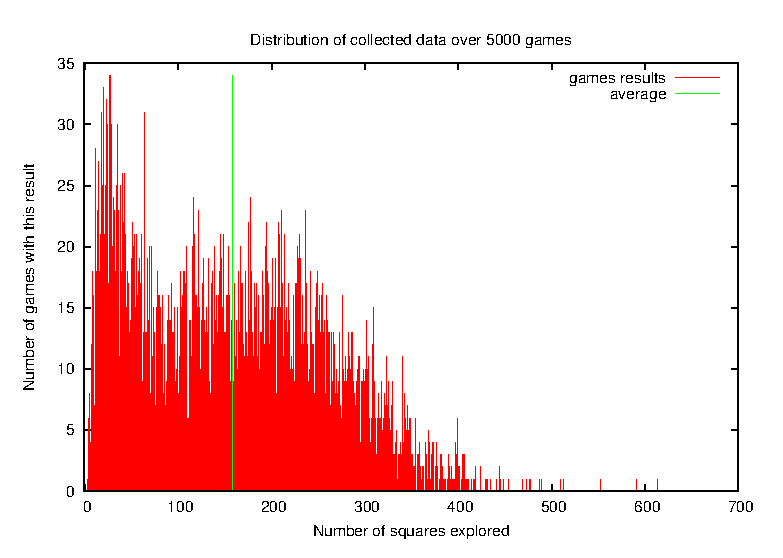
\includegraphics[width=\textwidth]{../images/impulse_graph.eps}}
	\caption{\label{fig:impulse_graph} Un exemple de fichier produit par impulse\_graph.sh}
\end{figure}

Lors de son exécution, ce script créé un dossier présent par bot trouvé dans
la base de donnée passée en paramètre et y ajoute tous les graphiques le
concernant. En conséquence, il est hautement recommandé que le dossier ne
contienne que la base de donnée lorsque celui-ci est exécuté.

\subsection{Graphiques comparant des bots}
Afin de comparer les performances des bots dans différents domaines, il est
possible d'utiliser le script \emph{move\_graph.sh}. Celui-ci génère des
graphiques pour les principales performances générées par les bots, les
résultats se présentent sous cette forme.

\begin{figure}[H]
  \center{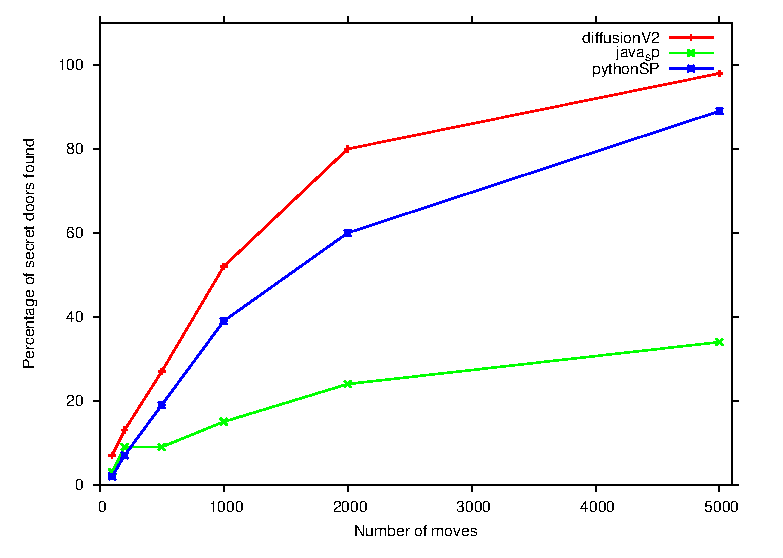
\includegraphics[width=\textwidth]{../images/move_graph.eps}}
  \caption{\label{fig:move_graph} Un exemple de fichier produit par move\_graph.sh}
\end{figure}

\subsection{Graphiques indiquant la répartition de différents objets}
Afin d'évaluer la répartition des portes secrètes ou des couloirs secrets,
quatre scripts sont mis à dispositions :

\begin{itemize}
\item 2d\_doors\_graph.sh
\item 3d\_doors\_graph.sh
\item 2d\_scorrs\_graph.sh
\item 3d\_scorrs\_graph.sh
\end{itemize}

Les scripts \emph{2d} produisent un graphique indiquant le nombre de cases
correspondant à la catégorie demandée sur chaque ligne et un autre par rapport
aux colonnes. 

\begin{figure}[H]
  \center{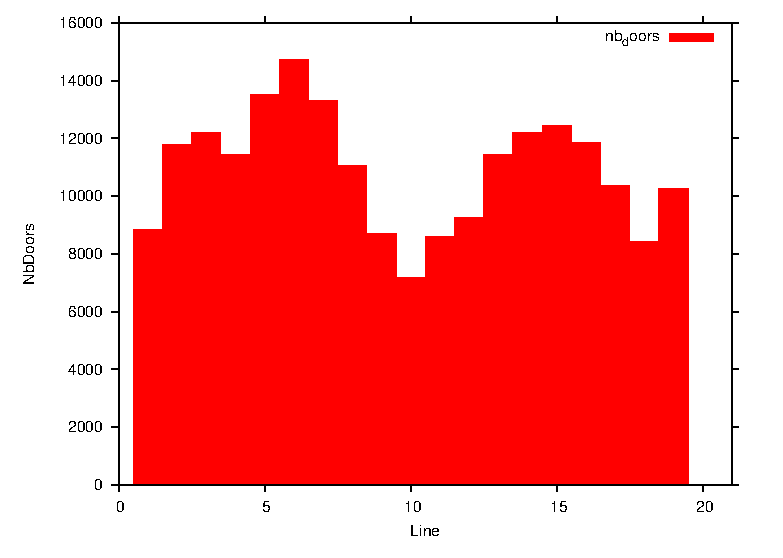
\includegraphics[width=\textwidth]{../images/2d_graph.eps}}
  \caption{\label{fig:2d_graph} Un exemple de graphique 2d}
\end{figure}


Les scripts \emph{3d} ne produisent pas de fichiers, mais ils ouvrent une
fenêtre gnuplot permettant de visualiser un graphe indiquant le nombre de cases
de la catégorie demandée pour chaque position. 

\begin{figure}[H]
  \center{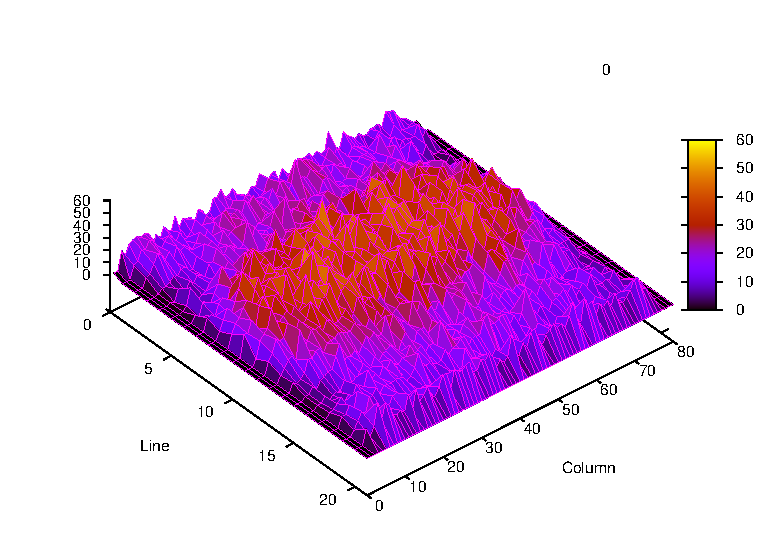
\includegraphics[width=\textwidth]{../images/3d_graph.eps}}
  \caption{\label{fig:3d_graph} Un exemple de visualisation en 3d}
\end{figure}

\chapter{Les bots}

\section{'Bot' contrôlé à la main}

L'interface développée ne permet plus de jouer au jeu à la main. Nous avons
alors développé un client adapté au protocole mis en place. Il s'agit du
programme \verb!bots/dummy-client.pl!. Il accepte les mêmes commandes que le jeu
original.

Ce client peut également être utilisé pour visualier une partie en cours jouée
par un bot. Cf. la section \emph{Voir ou revoir une partie}.


\section{Le starter package java}
Afin de pouvoir rapidement commencer à coder des bots, un \emph{starter package}
en java est fourni, les fonctionnalités fournies sont principalement la lecture
de la carte et la vérification de la validité des mouvements.
\\
Ce bot se contente de lister les actions possibles et d'en choisir une de façon
aléatoire, avec tout de même certaines actions prioritaires. Cette base permet
de pouvoir tester différentes stratégie sans avoir à implémenter à nouveau la
réception et l'envoi de message aux bots.

\section{Le bot diffusion}
Le principe de ce bot est d'établir des scores pour chaque cases et de diffuser
ensuite les valeurs à tous les voisins, ainsi la principale différence avec les
autres bots est que la complexité est bien plus élevée étant donnée que pour
choisir la prochaine action, il n'y a pas que le voisinage immédiat qui est
observé. Ce surcoût de temps permet en revanche d'avoir des meilleurs résultats
et la possibilité de modifier les scores facilement permet de changer les
objectifs en changeant uniquement des constantes.
\\
Une fois tous les scores calculés et la diffusion effectuée, l'action choisie
est celle ayant le score le plus élevé parmi celles qui sont autorisées. Ce bot
est donc totalement déterministe. Quelques attentions ont été portées à
l'optimisation afin de réduire légèrement le temps d'exécution, cependant, il
est certainement possible d'améliorer encore grandement les performances en
optimisant certaines parties du code.

\section{Le starter package python}

Ce bot propose un squelette pour l'interprétation des messages venant du jeu et un algorithme simple pour l'exploration 'rapide' d'un niveau en maintenant un compteur pour chaque case visitée. Le bot se déplace en priorité sur les cases les moins visitées.

\section{Le bot spécialisé}
Ce bot, écrit en python, n'a pas vocation à être utilisé dans des conditions
"normales" de jeu. C'est un bot dédié à la résolution optimale d'un problème
particulier : trouver, en un nombre de tours minimal, la porte secrète cachée
de façon aléatoire dans une salle carrée de taille 10x10. Une étude théorique
de ce problème a été réalisée et ce bot a pour but de s'approcher de la
solution optimale. Ceci permet d'effectuer une comparaison avec les autres
bots qui sont plus "généralistes".

Afin d'utiliser ce bot dans les bonnes conditions, il est nécessaire d'avoir
compilé une version du jeu dans laquelle le patch
\emph{patches/create\_level.patch} a été appliqué. Ce patch modifie le donjon
de telle sorte que le premier niveau ne contienne qu'une seule salle de la
forme décrite précédemment\footnote{ce niveau ne contient pas d'escalier pour descendre
dans les niveaux suivants}.

\chapter{Description technique}
\section{Les patchs du noyau de NetHack}
Afin de pouvoir facilement repartir d'une version originale du jeu, les
modifications du code de NetHack sont effectuées sous la forme de patchs. Il
est ainsi plus aisé de repérer les portions de codes qui ont été modifiées.

\subsection{Les patchs nécessaires}
Un ensemble de modifications du noyau de NetHack sont nécessaires au
fonctionnement des divers modules. Ces patchs sont regroupés dans le dossier
\emph{install} et définissent pour la plupart des \emph{hooks}, c'est-à-dire des
points d'entrée dans le cœur du code de NetHack. Ces points d'entrée sont en
fait des appels de fonctions dont le code est fourni dans les fichiers du
dossier \emph{src} et qui peuvent donc être modifiés indépendamment des patchs.

\subsection{Les patchs facultatifs}
Un ensemble de patchs a également été créé afin d'apporter des fonctionnalités
facultatives ou de restreindre la complexité de NetHack. Ces patchs se
trouvent dans le dossier \emph{patches} et peuvent être appliqués
indépendamment les uns des autres. Lors de l'installation, avec le script
\emph{nh-setup.sh}, il peut être choisi d'appliquer l'ensemble des patchs
listés dans le fichier \emph{patches/patch.conf} ou de choisir
individuellement ceux qui doivent être appliqués.
La plupart de ces patchs servent dans la définition d'un mode de jeu en
enlevant diverses contraintes de NetHack telles que la faim, les monstres, les
pièges ou les objets. Cela permet ainsi de construire des bots qui évoluent sur
une version simplifiée du jeu.

\section{Stockage des résultats}
Les résultats des parties sont stockés dans une base de données afin de ne pas perdre
trop d'informations et de pouvoir effectuer toute sorte de traitements dessus. Une vue
fournissant certains détails supplémentaires \footnote{Nombre de portes secrètes,
nombre de portes secrètes trouvées, nombre de couloirs secrets et nombre de couloirs
secrets trouvés.} est aussi disponible afin de faciliter l'utilisation de celle-ci.

\begin{figure}[H]
  \center{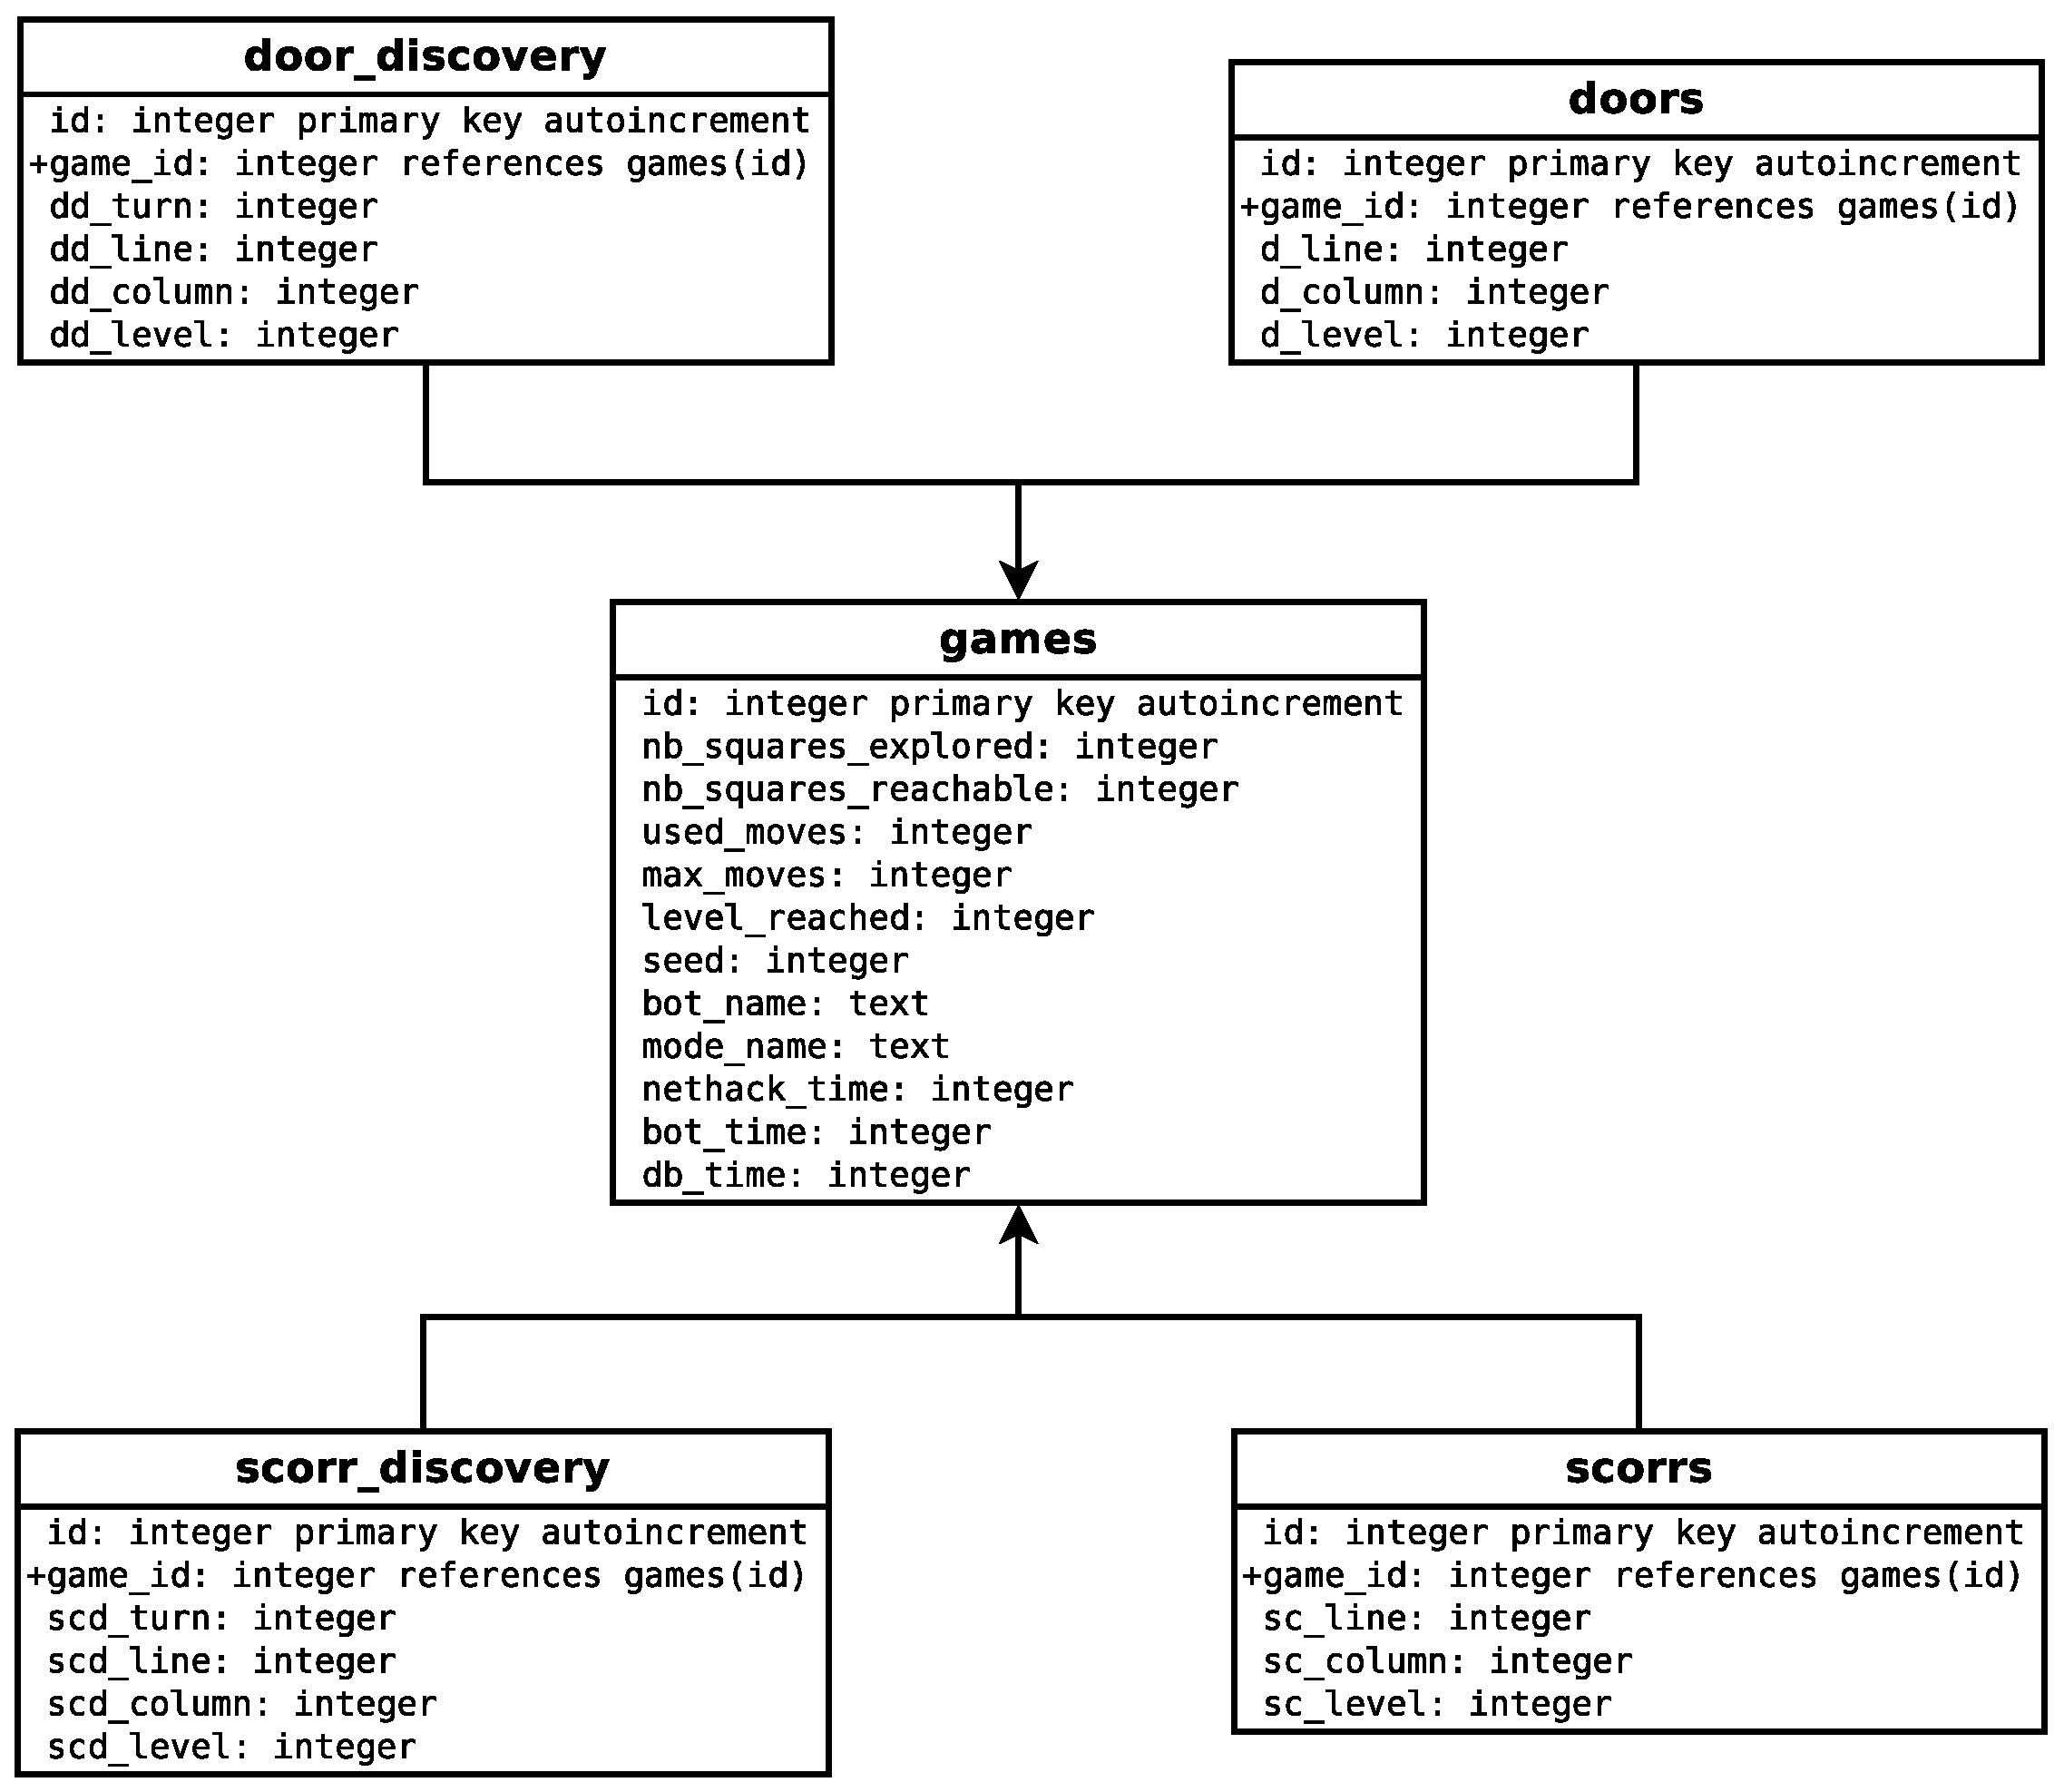
\includegraphics[width=\textwidth]{../images/schema_db.eps}}
	\caption{\label{fig:database} Schéma de la base de données}
\end{figure}

\chapter{Apporter ses propres modifications au code existant}
\section{Modifier du code source contenu dans les hooks}
Il est aisé de modifier du code source à l'intérieur des différents hooks
fournis car le script \emph{nh-setup.sh} permet de générer l'exécutable
\emph{nethack} en recompilant tous les fichiers sources nécessaires. Ainsi, il n'y aura
pas de modifications plus profonde à faire dans ce cas là. Cependant, si un
nouveau fichier est utilisé, il faudra néanmoins modifier le Makefile présent
dans le dossier \emph{install/nh/src} afin que les dépendances soient prises en
compte. Comme le fichier Makefile n'est pas recopié par défaut vers sa
destination, il faudra aussi spécifier à NetHack que l'on ne souhaite pas
réutiliser le code existant (ou copier le Makefile avant afin de gagner du temps
de compilation).


\section{Considérations pour la création de bots} \label{sec:creer-bot}

L'interface ne supporte pas les commandes commençant par le caractère '\verb!#!'. Ceci est dû au code original de NetHack qui cherche à réaliser des traitements particuliers pour ce type de commande (auto complétion, etc.) que nous n'avons pas jugé utile d'implémenter. Tout caractère '\verb!#!' est donc ignoré par l'interface.

Un bot peut envoyer plusieurs commandes à la fois ce qui peut se montrer utile pour diminuer le nombre d'échanges avec le jeu. Par exemple, envoyer les commandes '\verb!jjkl!' aura le même effet que d'envoyer chacune des lettres séparément et fera bouger le joueur deux fois vers le bas, une fois vers le haut et une fois vers la droite. Il est donc recommandé au développeur d'un bot de prendre en charge des patterns : \verb!oj! pour ouvrir une porte au sud, etc.

Quant au protocole concernant les échanges depuis l'interface vers le bot, nous avons établi les règles suivantes :
\begin{itemize}
	\item \verb!S! marque le début d'une transmission
	\item \verb!E! marque la fin d'une transmission et indique que l'interface attend une commande du client.
	\item \verb!g<x><y><glyph><code>! indique qu'un élément du jeu représenté
		par le caractère \verb!glyph! et ayant pour code identificateur
		\verb!code! se trouve aux coordonnées \verb!(x, y)!. \verb!x! et
		\verb!y! sont des entiers sur un octet; \verb!glyph! est un caractère;
		\verb!code! est un entier codé sur deux octets.
	\item \verb!C! indique que la carte doit être effacée. Un bot peut interpréter cette information comme étant un changement d'étage réussi s'il venait d'envoyer une commande descente ou montée d'escalier.
\end{itemize}

\section{Modifier les données stockées} \label{sec:modif-bdd}
Chaque table de la base de données possède son propre fichier \emph{.def} afin
d'ajouter un champ dans une table, il est donc nécessaire d'ajouter une entrée
dans ce fichier. Il faut aussi changer le nombre de champs de la table dans les
fichiers \emph{database\_manager.c} et \emph{game\_result.c}, il est aussi
nécessaire de fournir un getter pour chaque champs indiqué dans la base de
données. Cette architecture permet d'éviter trop de redondance de code en se
servant des macros. En revanche, pour ajouter une table, il est nécessaire de se
plonger plus profondément dans le code afin d'éviter tout désagrément, mais la
ligne de conduite principale reste d'ajouter un fichier \emph{.def}
\footnote{Attention aux dépendances dans le Makefile} et de copier le
comportement utilisé pour les autres tables.

\section{Créer un nouveau mode de jeu}
Les bases ont été posées afin de définir facilement des modes de jeu.
Un mode de jeu est défini de la façon suivante :
\begin{itemize}
		\item Un ensemble de modifications du jeu de base afin de
			rajouter/restreindre des fonctionnalités.
		\item Un ensemble de paramètres d'évaluation.
		\item Un ensemble d'objectifs ou conditions de fin de jeu.
		\item Un jeu d'actions autorisées pour les bots.
\end{itemize}

Les modifications du jeu de bases sont fournies sous la forme de patchs (ex :
un patch pour désactiver les montres, un autre pour désactiver la faim).
Chaque patch désactive une fonction particulière du jeu, ainsi différents
modes de jeu peuvent réutiliser les mêmes patchs. Par exemple, le mode de jeu
de recherche des portes secrètes nécessite la désactivation de tout ce qui
peut tuer le joueur c'est-à-dire les montres, les pièges, les objets et la
faim. Il serait aisé de définir un nouveau mode de jeu réexploitant les
différents patchs fourni, par exemple un mode combat dans lequel le but serait
de combattre des vagues de montres jusqu'à la mort pourrait nécessiter la
désactivation des autres sources de mort que les montres.

Pour définir un mode de jeu particulier voici ce qu'il faut faire :
\begin{itemize}
	\item Créer l'ensemble des patchs (cf. section numéro~\ref{sec:creer-patch} page~\pageref{sec:creer-patch}) modifiant le noyau de NetHack et nécessaires au mode de jeu.
	\item Ajouter des entrées dans la base de données pour les nouvelles données/statistiques à relever (cf. section numéro~\ref{sec:modif-bdd} page~\pageref{sec:modif-bdd}).
	\item Créer de nouveaux bots spécifiques à ce mode de jeu (cf. section numéro~\ref{sec:creer-bot} page~\pageref{sec:creer-bot}).
	\item Modifier si besoin le middleman afin, par exemple, d'ajouter des choses au protocole de communication entre les bots et le noyau de NetHack.
\end{itemize}

\section{Créer un patch} \label{sec:creer-patch}

\textbf{\_\_Exemple de successions de commandes permettant de créer un patch\_\_}.

\section{Ajouter des niveaux spéciaux}

\url{http://nethack.wikia.com/wiki/Des-file\_format#SUBROOM}

\chapter{Dysfonctionnements connus}
\section{Sémaphore bloquée de façon permanente}
Lorsqu'un utilisateur tue un processus de NetHack, le processus peut se terminer
alors qu'il est dans une zone critique, il ne libère donc pas l'accès à la base
de données, une solution peut être implémentée à l'aide d'un gestionnaire de
signal, cependant au vu des appels à une bibliothèque externe, il est possible
que cela ne suffise pas. Actuellement, la meilleure solution dans ce cas est
d'effacer le sémaphore afin que les nouveaux processus de NetHack ne soient pas
bloqués lorsqu'ils tentent d'écrire dans la base de données. Sur certains
systèmes, les fichiers de sémaphore nommées peuvent être trouvés dans 
\emph{/dev/shm/}, dans le cas où l'utilisateur ne parvient pas à trouver
comment effacer les sémaphore nommées, il existe deux autres solutions :
renommer la base de données afin de changer le nom de sémaphore associé ou
redémarrer \footnote{attention, si la base de données est dans les fichiers
temporaires, il est 
conseillé de la déplacer avant}.

\end{document}
